%% Copernicus Publications Manuscript Preparation Template for LaTeX Submissions
%% ---------------------------------
%% This template should be used for copernicus.cls
%% The class file and some style files are bundled in the Copernicus Latex Package, which can be downloaded from the different journal webpages.
%% For further assistance please contact Copernicus Publications at: production@copernicus.org
%% https://publications.copernicus.org/for_authors/manuscript_preparation.html

%% copernicus_rticles_template (flag for rticles template detection - do not remove!)

%% Please use the following documentclass and journal abbreviations for discussion papers and final revised papers.

%% 2-column papers and discussion papers
\documentclass[gc, manuscript]{copernicus}



%% Journal abbreviations (please use the same for discussion papers and final revised papers)


% Advances in Geosciences (adgeo)
% Advances in Radio Science (ars)
% Advances in Science and Research (asr)
% Advances in Statistical Climatology, Meteorology and Oceanography (ascmo)
% Annales Geophysicae (angeo)
% Archives Animal Breeding (aab)
% ASTRA Proceedings (ap)
% Atmospheric Chemistry and Physics (acp)
% Atmospheric Measurement Techniques (amt)
% Biogeosciences (bg)
% Climate of the Past (cp)
% DEUQUA Special Publications (deuquasp)
% Drinking Water Engineering and Science (dwes)
% Earth Surface Dynamics (esurf)
% Earth System Dynamics (esd)
% Earth System Science Data (essd)
% E&G Quaternary Science Journal (egqsj)
% European Journal of Mineralogy (ejm)
% Fossil Record (fr)
% Geochronology (gchron)
% Geographica Helvetica (gh)
% Geoscience Communication (gc)
% Geoscientific Instrumentation, Methods and Data Systems (gi)
% Geoscientific Model Development (gmd)
% History of Geo- and Space Sciences (hgss)
% Hydrology and Earth System Sciences (hess)
% Journal of Bone and Joint Infection (jbji)
% Journal of Micropalaeontology (jm)
% Journal of Sensors and Sensor Systems (jsss)
% Magnetic Resonance (mr)
% Mechanical Sciences (ms)
% Natural Hazards and Earth System Sciences (nhess)
% Nonlinear Processes in Geophysics (npg)
% Ocean Science (os)
% Primate Biology (pb)
% Proceedings of the International Association of Hydrological Sciences (piahs)
% Scientific Drilling (sd)
% SOIL (soil)
% Solid Earth (se)
% The Cryosphere (tc)
% Weather and Climate Dynamics (wcd)
% Web Ecology (we)
% Wind Energy Science (wes)


%% \usepackage commands included in the copernicus.cls:
%\usepackage[german, english]{babel}
%\usepackage{tabularx}
%\usepackage{cancel}
%\usepackage{multirow}
%\usepackage{supertabular}
%\usepackage{algorithmic}
%\usepackage{algorithm}
%\usepackage{amsthm}
%\usepackage{float}
%\usepackage{subfig}
%\usepackage{rotating}

% Pandoc citation processing

% The "Technical instructions for LaTex" by Copernicus require _not_ to insert any additional packages.
%
\usepackage{algorithmic}
\usepackage{algorithm}


\begin{document}

\title{Management induced changes of soil organic carbon on global croplands}


\Author[1, 3]{Kristine}{Karstens}
\Author[1]{Benjamin Leon}{Bodirsky}
\Author[1]{Jan Philipp}{Dietrich}
\Author[2]{Marta}{Dondini}
\Author[1]{Jens}{Heinke}
\Author[2]{Matthias}{Kuhnert}
\Author[1]{Christoph}{Müller}
\Author[1]{Susanne}{Rolinski}
\Author[2]{Pete}{Smith}
\Author[1]{Isabelle}{Weindl}
\Author[1, 3]{Hermann}{Lotze-Campen}
\Author[1]{Alexander}{Popp}


\affil[1]{Potsdam Institute for Climate Impact Research (PIK), Member of the Leibniz Association, P.O. Box 60 12 03, 14412 Potsdam, Germany}
\affil[2]{Institute of Biological \& Environmental Sciences, University of Aberdeen, Aberdeen, UK}
\affil[3]{Humboldt-Universität zu Berlin, Department of Agricultural Economics, Unter den Linden 6, 10099 Berlin, Germany}

\runningtitle{R Markdown Template for Copernicus}

\runningauthor{Nüst et al.}


\correspondence{Kristine\ Karstens\ (\href{mailto:kristine.karstens@pik-potsdam.de}{\nolinkurl{kristine.karstens@pik-potsdam.de}})}



\received{}
\pubdiscuss{} %% only important for two-stage journals
\revised{}
\accepted{}
\published{}

%% These dates will be inserted by Copernicus Publications during the typesetting process.


\firstpage{1}

\maketitle


\begin{abstract}
Soil organic carbon (SOC) is one of the largest terrestrial carbon stocks on Earth. The first meter of the Earths soils profile stores three times as much carbon as the vegetation and twice the amount of C in the atmosphere. SOC has been depleted by anthropogenic land cover change and agricultural management. However, the latter has so far not been well represented in global carbon stock assessments. While SOC models often simulate detailed biochemical processes that lead to the accumulation and decay of SOC, the management decisions driving these biophysical processes are still little investigated at the global scale. Here we develop a spatial explicit data set for agricultural management on cropland, considering crop production levels, residue returning rates, manure application, and the adoption of irrigation and tillage practices. We combine it with the IPCC Tier 2 steady-state soil model to create a half-degree resolution data set of SOC stocks and SOC stock changes for the first 30 cm of mineral soils. We estimate that due to arable farming, soils have lost around 26 GtC relative to a counterfactual natural state in 1975. Yet, within the period 1975--2010 this SOC debt has been decreasing again by a net quantity of 4 Gt SOC, which can be mainly traced back to an increased input of C in crop residues due to higher crop productivity. We also find that SOC is very sensitive to management decisions such as residue returning indicating the necessity to incorporate better management data in soil model simulations.
\end{abstract}




\newpage

\introduction

Soil Organic Carbon (SOC), the amount of organic carbon stored in the Earth's soil, is the largest terrestrial organic carbon pool. It exceeds the carbon in the atmospheric and vegetation pools multiple times \citep{batjes_total_1996}. Even small changes in processes affecting SOC lead therefore to substantial shifts in the terrestrial carbon cycle and influence the amount of CO\textsubscript{2} in the atmosphere \citep{friedlingstein_global_2019, minasny_soil_2017}. The specific amount of carbon stored in soils globally is quantified with estimates ranging from 1500 to 2400 GtC for the first meter of the soil profile \citep{batjes_total_1996, sanderman_soil_2017}.

Natural properties like climatic, biophysical, and landscape characteristics clearly play the most important roles to determine SOC variations over space and time. Recent studies have focused on the evaluation of total SOC stocks of the world as well as on the spatial disaggregation of soil properties such as SOC content \citep{batjes_harmonized_2016, hengl_soilgrids250m_2017, fao_global_2018}. However, these studies often do not include human interventions, like land cover change and agricultural management, in their analysis. Compared to climatic and geological drivers, they alter terrestrial carbon pools over much shorter time scales and are currently one of most dominant drivers of SOC changes on managed land.

The anthropogenic impact can be measured by the SOC debt (also referred to as SOC component of land-use change emissions), which is the amount of organic carbon soils have lost under cultivation compared to a potential natural vegetated state. Sanderman et al.~\citeyearpar{sanderman_soil_2017} identified the anthropogenic SOC debt for the first meter of the soil profile due to land cover change at around 116 GtC (37 GtC for the first 30 cm), compared to previous estimates of 60--130 GtC for the first meter \citep{lal_world_2001}.

Global assessments of the carbon cycle via dynamic global vegetation models (DGVMs) and Earth System Models (ESMs) or bookkeeping models (BKMs) have analyzed SOC losses as part of a comprehensive evaluation of the global carbon budget and land-use change (LUC) emissions \citep{friedlingstein_global_2019}. While providing estimates of the magnitude of SOC losses due to land cover change, most models lack a detailed consideration of agricultural management. Earlier DGVM and ESM based assessments only considered changes in land cover, but ignored the removal of biomass at harvest \citep{strassmann_simulating_2008, betts_climate_2015}. BKMs are designed to estimate LUC related emissons but ignore changes in SOC due to climate change, CO\textsubscript{2} fertilization, and agricultural management \citep{friedlingstein_global_2019, houghton_carbon_2012, hansis_relevance_2015}.

Managed agricultural systems were introduced in greater detail to DGVMs and ESMs to improve the assessment of the terrestrial carbon balance \citep[e.g.~][]{bondeau_modelling_2007, lindeskog_implications_2013}. Pugh et al.~\citeyearpar{pugh_simulated_2015} explicitly consider agricultural management in the form of tillage, irrigation and biomass extraction at harvest, but worked with stylized scenarios rather than with historic management data. They also showed the importance of accounting for the land-use history, as many carbon emissions from agricultural soils are caused by historic LUC and the slow decline of SOC under cropland before it reaches a new equilibrium.

In global-scale carbon cycle assessments, management systems are typically represented as spatially explicit patterns that are static in time (e.g.~growing seasons \citep{portmann_mirca2000global_2010} multiple cropping systems \citep{waha_multiple_2020}, irrigation systems \citep{jagermeyr_water_2015}) or as stylized scenarios \citep[e.g.~][\citet{lutz_simulating_2019}]{pugh_simulated_2015}.

More data sets on spatially explicit agricultural management time series with global coverage become available (e.g.~on tillage systems, see \citep{porwollik_generating_2018}, \citep{prestele_spatially_2018}) and model approaches are increasingly developed to project the dynamics of management systems into the future (e.g.~\citep{iizumi_modeling_2019}, \citep{minoli_modelling_2019}), but have --- to our knowledge --- not found their way into comprehensive assessments of the terrestrial carbon cycle in DGVMs and BKMs.

Field-scale models \citep[\citet{coleman_simulating_1997}, \citet{smith_estimating_2010}, \citet{taghizadeh-toosi_c-tool_2014}]{del_grosso_simulated_2001} are able to better account for historic agricultural management if detailed information on crop yield levels, fertilizer inputs and various other on-farm measures is available for the studied sites. However, due to the lack of comprehensive global management data as input to these models, scaling up to the global domain remains a complex challenge.

The objective of our study is to provide the first global, spatially explicit SOC and SOC debt map that considers spatially explicit and time-variant historic agricultural management. To achieve this objective we create and provide a comprehensive data set of the global gridded management time series data, including crop production levels, residue returning rates, manure application, and the adoption of irrigation and tillage practices. We simulate SOC stocks, dynamics and the SOC debt for 1975--2010. Using a scenario analysis, we decompose the contribution of different management activities.
\newpage

\hypertarget{methods}{%
\section{Methods}\label{methods}}

In Sect. \ref{sec:carbonbudget} we introduce the basic concept of SOC dynamics as applied in this study and explained in more detail within the refinement of the IPCC guidelines vol.~4 \citep{calvo_buendia_ipcc_2019}. We additionally describe how we configured and extended the steady-state method (for model code see \citep{karstens_mrsoil_2020}. In Sect. \ref{sec:tier1} we shortly refer to the concept of stock change factors as outlined in the Tier 1 approach of the IPCC guidelines \citep{eggleston_ipcc_2006, calvo_buendia_ipcc_2019}.
Section \ref{sec:agrimanagement} provides a detailed description of the global, gridded management data used to drive the model, including crop production levels, residue input rates, manure amendments, and the adoption of irrigation and tillage practices \citep[for model code see][]{bodirsky_mrcommons_2020}. In Sect. \ref{sec:scenarios} we define the scenarios used to complement our historic model results.

\hypertarget{sec:carbonbudget}{%
\subsection{SOC stocks and stock changes following the steady-state method}\label{sec:carbonbudget}}

Following the Tier 2 steady-state approach of the refinement of the IPCC guidelines vol.~4 \citep{calvo_buendia_ipcc_2019}; referred to as \textit{steady-state method} in the following), we estimate soil organic carbon (\(SOC\)) stocks and their change over time for cropland at half-degree resolution from 1975 to 2010. We restrict our analysis to the first 0-30 cm of the soil profile. Moreover, we assume the current \(SOC\) state converges towards a steady state, which itself depends on biophysical, climatic and agronomic conditions.
Therefore, we take the following three steps for each year of our simulation period:
(1) We calculate annual land-use type-specific steady states and decay rates for \(SOC\) stocks (Sect. \ref{sec:steadystates});
(2) we account for land conversion by transferring \(SOC\) from and to natural vegetation (Sect. \ref{sec:carbontransfer}),
(3) we estimate \(SOC\) stocks and changes based on the stocks of the previous time step, the steady state stocks and the decay rate (Sect. \ref{sec:totalsoc}).
To initialize the first year of our simulation period we use a spin-up period of 74 years (Sect. \ref{sec:initsoc}).

\hypertarget{sec:steadystates}{%
\subsubsection{Steady-state SOC stocks and decay rates}\label{sec:steadystates}}

In a simple first order kinetic approach the steady-state soil organic carbon stocks \(SOC^{\mathrm{eq}}\) are given by
\begin{equation}
SOC^{\mathrm{eq}}_{i,t,sub,lu} =\frac{C^{\mathrm{in}}_{i,t,sub,lu}}{k_{i,t,sub,lu}}
\label{eq:inoutflow}
\end{equation}
with \(C^{\textrm{in}}\) being the carbon inputs to the soil, \(k\) denotes the soil organic carbon decay rate. This equation is valid for all grid cells \(i\) and all years \(t\). We use the steady-state method for our calculations, which assumes three soil carbon sub-pools \(sub\) (active, slow and passive) and interactions between them, following the approach in the Century model \citep{parton_analysis_1987}. Annual carbon inflow to each sub-pool and annual decay rates of each sub-pool are land-use type \(lu\) specific.
We distinguish two land-use types: cropland and uncropped land under potential natural vegetation as representative for all other land-use types including forestry and pastures (referred to as natural vegetation in the following).

Carbon inputs for cropland are below- and above-ground residues left or returned to the field (see Sect. \ref{sec:residues}) and manure inputs (see Sect. \ref{sec:livstmanure}); for natural vegetation litterfall including fine root turnover \citep{schaphoff_lpjml4_2018} is the only source of carbon inflow to the soil. Following the IPCC guidelines \citep{calvo_buendia_ipcc_2019}, carbon inputs are disaggregated into metabolic and structural components depending on their lignin and nitrogen content. For each component the sum of all carbon input sources is allocated to the respective \(SOC\) sub-pools via transfer coefficients. This implies that both the amount of carbon and its structural composition determine the effective inflow into the different pools. Data sources for all considered carbon inputs as well as for lignin and nitrogen content are listed in Table \ref{tab:datasourceinputs}.

  \begin{table*}[h]
  \caption{Type and data sources for carbon inputs and parameterization to different land-use types }
  \begin{tabular}{p{0.15\textwidth} p{0.20\textwidth} p{0.20\textwidth} p{0.35\textwidth}}
  \tophline
  \textbf{land-use types}   & \textbf{source of carbon inputs} & \textbf{data source} & \textbf{nitrogen and lignin content} \\
  \middlehline
  \multirow{3}{*}{Cropland} & above-ground residues, & \multirow{3}{*}{\begin{minipage}[t]{0.35\columnwidth}\raggedright
                                                                      \citet{faostat_faostat_2016}, \\
                                                                      \citet{schaphoff_lpjml4_2018},\\
                                                                      \citet{weindl_livestock_2017} \end{minipage}} & 
                                                      \multirow{3}{*}{\begin{minipage}[t]{0.35\columnwidth}\raggedright
                                                                      LG:C generic values according to Table 5.5B,\\
                                                                      5.5C from IPCC \citep{calvo_buendia_ipcc_2019},\\
                                                                      crop-specific N:C from \citet{bodirsky_n2o_2012}
                                                                      \end{minipage}} \\
                            & below-ground residues, &  &  \\
                            & manure                &  &  \\ 
                            \hline
  Natural vegetation        & annual litterfall &  \citet{schaphoff_lpjml4_2018}
                            & \begin{minipage}[t]{0.35\columnwidth}\raggedright\strut 
                                IPCC \citep{calvo_buendia_ipcc_2019} and\\ 
                                CENTURY (\citep{century_model_2000}) \strut \end{minipage}\tabularnewline
 \bottomhline
 \end{tabular}
 \label{tab:datasourceinputs}
 \belowtable{}
 \end{table*}

The sub-pool specific decay rates \(k_{sub}\) are influenced by climatic conditions, biophysical and biochemical soil properties as well as management factors that all vary over space (\(i\)) and time (\(t\)). Following the steady-state method \citep{calvo_buendia_ipcc_2019}, we consider temperature (\(temp\)), water (\(wat\)), sand fraction (\(sf\)) and tillage (\(till\)) effects to account for spatial variation of decay rates. Thus, \(k_{sub}\) are given by

\begin{equation}
\begin{aligned}
& k_{i,t,\mathrm{active},lu}  & = &~ k_{\mathrm{active}}  ~ &\cdot~ temp_{i,t} ~ &\cdot~ wat_{i,t,lu} ~ &\cdot~ till_{i,t,lu} ~ & \cdot~ sf_{i}\\
& k_{i,t,\mathrm{slow},lu}    & = &~ k_{\mathrm{slow}}    ~ &\cdot~ temp_{i,t} ~ &\cdot~ wat_{i,t,lu} ~ &\cdot~ till_{i,t,lu} ~ &\\
& k_{i,t,\mathrm{passive},lu} & = &~ k_{\mathrm{passive}} ~ &\cdot~ temp_{i,t} ~ &\cdot~ wat_{i,t,lu} ~ & ~ & 
\label{eq:decayrates}
\end{aligned}.
\end{equation}

For natural vegetation, we assume rainfed and non-tilled conditions, whereas for cropland, we distinguish the effect of different tillage (see Sect. \ref{sec:tillage}) and irrigation (see Sect. \ref{sec:irrigation}) practices on decay rates. We calculated area weighted means for \(till\) and \(wat\) on cropland for each grid cell, using area shares for the different tillage and irrigation pratices. Data sources as well as used parameters for the different decay drivers for all land-use types are listed in Table \ref{tab:datasourcedecay}; equations are displayed by equation 5.0B--5.0F in Calvo Buendia et al.~\citeyearpar{calvo_buendia_ipcc_2019}.

 \begin{table*}[h]
 \caption{Type and data sources for carbon inputs to different land-use types}
 \begin{tabular}{l l l l}
 \tophline
  land-use types   & type of decay driver & parameter use to represent driver & data source \\
 \middlehline
 \multirow{2}{*}{all} & Soil quality & Sand fraction of the first 0-30 cm 
                                     & \citet{hengl_soilgrids250m_2017} \\
                      \cline{2-4}
                      
                      & Mircobial activity & air temperature & \citet{harris_version_2020} \\
                      \cline{2-4}
                      
                      & Water restriction & precipitation \& potential evapotranspiration & \citet{harris_version_2020} \\
                      \cline{1-4}
\multirow{2}{*}{\begin{minipage}[t]{0.2\columnwidth}\raggedright\strut Cropland\\(additionally)\strut\end{minipage}} & Water restriction*  & irrigation  & Sect. \ref{sec:irrigation} \\ 
                      \cline{2-4}
                      
                      & Soil disturbance & tillage & Sect. \ref{sec:irrigation} \\
 \bottomhline
 \end{tabular}
 \belowtable{}
 \label{tab:datasourcedecay}
 \end{table*}

\hypertarget{sec:carbontransfer}{%
\subsubsection{SOC transfer between land-use types}\label{sec:carbontransfer}}

We calculate \(SOC\) stocks based on the area shares of land-use types (\(lu\)) within our grid cells (\(i\)). If land is converted from one land-use type \(lu=\{crop,natveg\}\) into the other \(!lu=\{natveg,crop\}\), a respective share of the \(SOC\) is reallocated. We account for land conversion at the beginning of each time step \(t\) by calculating a preliminary stock \(SOC_{t^*}\) via

\begin{equation}
SOC_{i,t^*,sub,lu} = SOC_{i,t-1,sub,lu} - \frac{SOC_{i,t-1,sub,lu}}{A_{i,t-1,lu}} \cdot  AR_{i,t,lu} + \frac{SOC_{i,t-1,sub,!lu}}{A_{i,t-1,!lu}} \cdot  AE_{i,t,lu}
\label{eq:ctransfer}
\end{equation}

with \(A_{lu}\) being the land-use type specific areas, \(AR_{lu}\) and \(AE_{lu}\) the area reduction resp. area expansion of the two land-use types. Data sources and methodology on land-use states and changes are described in Sect. \ref{sec:landuse}.

\hypertarget{sec:totalsoc}{%
\subsubsection{Total SOC stocks and stock changes}\label{sec:totalsoc}}

\(SOC\) converge towards the calculated steady-state stock \(SOC^{\mathrm{eq}}\) for each grid cell \(i\), each annual time step \(t\), each land-use type \(lu\) and each sub-pool \(sub\) like

\begin{equation}
SOC_{i,t,sub,lu} = SOC_{i,t^*,sub,lu} + (SOC^{\mathrm{eq}}_{i,t,sub,lu} - SOC_{i,t^*,sub,lu}) \cdot k_{i,t,sub,lu} \cdot 1\unit{a}.
\label{eq:SOCstate}
\end{equation}

Note that the decay rates have to be multiplied by one year (\(1a\)) to form a dimensionless factor.
Reformulating this equation, we obtain a mass balance equation as follows

\begin{equation}
SOC_{i,t,sub,lu} = SOC_{i,t^*,sub,lu} - \underbrace{SOC_{i,t^*,sub,lu} \cdot k_{i,t,sub,lu} \cdot 1\unit{a}}_{\text{outflow}} + \overbrace{SOC^{\mathrm{eq}}_{i,t,sub,lu} \cdot k_{i,t,sub,lu} \cdot 1\unit{a}}^{\text{input (using equation (1))}}.
\label{eq:steadystate2budget}
\end{equation}

The global \(SOC\) stock for each time step \(t\) can then be calculated via

\begin{equation}
SOC_{t} = \sum_{i} \underbrace{\sum_{lu} \overbrace{\sum_{sub} SOC_{i,t,sub,lu}}^{\text{$SOC_{i,t,lu}$ -- land-use type specific SOC stock within cell}}}_{\text{$SOC_{i,t}$ -- total SOC stock within cell}}.
\label{eq:totalstock}
\end{equation}

According to the IPCC guidelines \(SOC\) changes can be expressed as the difference of two consecutive years \citep[see Eq. 5.0A in][]{calvo_buendia_ipcc_2019}. This, however, will also include naturally occurring changes due to climatic variation over time. For our study, we defined the absolute and relative SOC changes in relation to a potential natural state \(SOC^{\mathrm{pnv}}\) under the same climatic conditions in grid cell \(i\) at time \(t\), that is based on the natural vegetation \(SOC\) calculations as defined above without accounting for land conversion from cropland at any time. The absolute changes \(\Delta SOC\) and relative changes \(F^{\mathrm{SCF}}\) are thus given by

\begin{equation}
\Delta SOC_{i,t} = SOC_{i,t} - SOC^{\mathrm{pnv}}_{i,t}\qquad \text{and} \qquad  F^{\mathrm{SCF}}_{i,t} = \frac{SOC_{i,t}}{SOC^{\mathrm{pnv}}_{i,t}} .
\label{eq:stockdiff}
\end{equation}

Note that the absolute changes \(\Delta SOC\) can be also interpreted as the SOC debt \citep{sanderman_soil_2017} due to human cropping activities; whereas relative changes \(F^{\mathrm{SCF}}\) can be considered stock change factors as defined within the IPCC guidelines of 2006 \citep{eggleston_ipcc_2006}. Moreover, \(\Delta SOC\) is equivalent to the negated cumulative SOC component of human land-use change emissions \citep{pugh_simulated_2015}.

\hypertarget{sec:initsoc}{%
\subsubsection{Initialization of SOC pools}\label{sec:initsoc}}

To initialize all SOC sub-pools we assume that cropland and natural vegetation are in a land-use type specific steady state for the initialization year 1901. While land-use, climate and litter input information are available from 1901, agricultural management data on residue and manure inputs are held constant at the level of 1965. After a spin-up period of 64 years (1901-1965) with constant agricultural input data, we run the model for additional 10 years with historic input data and start analyzing results from 1975 onwards. Irrigation areas are part of the land-use data set and therefore dynamic from 1901 on, whereas data on no-tillage area is only available after 1974.

\hypertarget{sec:tier1}{%
\subsection{SOC stocks and stock changes following Tier 1}\label{sec:tier1}}

Additionally to the steady-state method \citep{calvo_buendia_ipcc_2019} and the detailed analysis of management data coming with it, SOC changes can be estimated using the IPCC Tier 1 approach of IPCC guidelines \citep{eggleston_ipcc_2006, calvo_buendia_ipcc_2019}. Here, stocks are calculated via stock change factors (\(F^{\mathrm{SCF}}\)) given by the IPCC for the topsoil (0-30 cm) and based on observational data. Estimates of \(F^{\mathrm{SCF}}\) are differentiated by different crops, management and input systems (here summarized under \(m\)) reflecting different dynamics under changed in- and outflows without explicitly tracking these. Moreover, estimates of \(F^{\mathrm{SCF}}\) vary for different climatic zones (\(c\)) specified by the IPCC (see Fig. \ref{fig:CLIMzone}). The actual \(SOC\) stocks are thus calculated based on a given reference stock \(SOC^{\mathrm{ref}}\) by

\begin{equation}
SOC_{i,t} = \sum_{c,m} T_{c,i} \cdot SOC^{\mathrm{ref}}_{i,t} \cdot F^{\mathrm{SCF}}_{c,m}
\label{eq:tier1}
\end{equation}

with \(T_{c,i}\) being the translation matrix for grid cells \(i\) into corresponding climate zones \(c\). For this analysis, we use the default \(F^{\mathrm{SCF}}\) from the Tier 1 method of Eggleston et al.~\citeyearpar{eggleston_ipcc_2006} and Calvo Buendia et al.~\citep{calvo_buendia_ipcc_2019} as a comparison and consistency check for our more detailed Tier 2 steady-state approach.

\hypertarget{sec:agrimanagement}{%
\subsection{Agricultural management data at 0.5 degree resolution}\label{sec:agrimanagement}}

We compile country-specific FAO production and cropland statistics \citep{faostat_faostat_2016} to a harmonized and consistent data set. The data is prepared in 5-year time steps from 1965 to 2010, which restricts our analysis to the time span from 1975 to 2010 (after a spin-up phase from 1901-1974). For all the following data, if not declared differently, we interpolate values linearly between the time steps and keep them constant before 1965.

\hypertarget{sec:landuse}{%
\subsubsection{Land use and land-use change}\label{sec:landuse}}

Land-use patterns are based on the Land-Use Harmonization 2 \citep{hurtt_harmonization_2020} data set, which we sum up from quarter-degree to half-degree resolution. We disaggregate the physical area of the five different cropland subcategories (c3ann, c3per, c4ann, c4per, c3nfx) of LUH2 into our 17 crop groups \citep[see FAO2LUH2MAG\_croptypes.csv in][]{bodirsky_mrcommons_2020}, applying the relative shares for each grid cell based on the country- and year-specific area harvested shares of FAOSTAT data \citep{faostat_faostat_2016}. By calculating country-specific multicropping factors using FAOSTAT data, we are able to compute crop-group specific area harvested on grid cell level.
Land-use transitions are calculated as net area differences of the land-use data at half-degree resolution, considering no split up into crop-group specific areas but only total cropland and natural vegetation areas.

\hypertarget{sec:residues}{%
\subsubsection{Crop and crop residues production}\label{sec:residues}}

Crop production patterns are compiled crop group specific using half-degree yield data from LPJmL \citep{schaphoff_lpjml4_2018} as well as half-degree cropland patterns (see Sect. \ref{sec:landuse}). We calibrate cellular yields with a country-level calibration factor for each crop group to meet historic FAOSTAT production \citep{faostat_faostat_2016}. By using physical cropland areas in combination with harvested areas, we account for multiple cropping systems as well as for fallow land.

Crop residue production and management is based on a revised methodology of Bodirsky et al.~\citeyearpar{bodirsky_n2o_2012} and key aspects are explained here given its central role for soil carbon modeling. Starting from harvested crop production (\(CP\)) estimates and their respective harvested crop area (\(CA\)), we estimate above-ground (\(AGR\)) and below-ground (\(BGR\)) residual biomass using crop group (\(cg\)) specific harvest index values (\(HI\)) and root:shoot ratios (\(RS\)) as follows

\begin{equation}
\begin{aligned}
AGR_{i,t,cg} & = CP_{i,t,cg} \cdot HI^{\mathrm{prod}}_{cg} + CA_{i,t,cg} \cdot HI^{\mathrm{area}}_{cg}
\qquad & \textrm{and} \\
BGR_{i,t,cg} & = (CP_{i,t,cg} + AGR_{i,t,cg}) \cdot RS_{cg} \qquad                                            & \forall\quad cg, i, t.
\label{eq:resbiomass}
\end{aligned}
\end{equation}

Following the IPCC guidelines, we split the harvest index into a production (\(HI^{\mathrm{prod}}\)) and an area dependent (\(HI^{\mathrm{area}}\)) fraction \citep{eggleston_ipcc_2006}. Deviating from Bodirsky et al.~\citeyearpar{bodirsky_n2o_2012} we use harvested instead of physical crop area to account for increased residue biomass due to multiple cropping and decreased residue amounts due to fallow land. We assume that all \(BGR\) are left in the soil, whereas \(AGR\) can be burned or harvested for other purposes such as feeding animals \citep{weindl_livestock_2017}, fuel or for material use.

A country-specific fixed share of the \(AGR\) is assumed to be burned on field depending on the per-capita income of the country. Following Smil \citeyearpar{smil_nitrogen_1999} we assume a burn share of \(25\%\) for low-income countries according to World Bank definitions (\(<\,1000\,\tfrac{USD}{yr\,cap}\)), 15\% for high-income (\(>\,10000\,\tfrac{USD}{yr\,cap}\)) and linearly interpolate shares for all middle-income countries depending on their per-capita income. Depending on the crop group, 80--90\% of the carbon in the crop residues burned in the fields is lost within the combustion process \citep{eggleston_ipcc_2006}.

From our 17 crop groups, we compile four residue groups (straw, high- and low-lignin residues, residues without dual use), of which the first three are taken away from the field for other purposes (see mappingCrop2Residue.csv in Bodirsky et al.~\citeyearpar{bodirsky_mrcommons_2020}. Residue feed demand for five different livestock groups is based on country-specific feed baskets \citep[see][]{weindl_livestock_2017}, that differentiate between the residue groups and take available \(AGR\) biomass as well as livestock productivity into account. We estimate a material-use share for the straw-residue group of 5\% and a fuel-share of 10\% for all used residue groups in low-income countries. For high-income countries, no withdrawal for material or fuel use is assumed, and use shares of middle-income countries are linearly interpolated based on per-capita income, following the same rationale as for the share of burnt residues described above. The remaining \(AGR\) as well as all \(BGR\) are expected to be left on the field. We limit high residue return rates to at most \(10\unit{tC\,ha}^{-1}\) in order to correct for outliers.

To transform dry matter estimates into carbon and nitrogen, we compiled crop-group and plant-part specific carbon resp. nitrogen to dry matter (c/dm, n/dm) ratios (see \ref{tab:c2dm}).

\hypertarget{sec:livstmanure}{%
\subsubsection{Livestock distribution and manure excretion}\label{sec:livstmanure}}

Manure especially from ruminants is often excreted at pastures and rangelands, but due to the intensification of livestock systems at the present day a lot of the manure has to be stored and can be applied on croplands. We assume that manure application happens at its excretion place, so that the livestock distribution is the driving factor of the spatial pattern of manuring.

To disaggregate country level FAOSTAT livestock production data to half-degree resolution, we use the following rule-based assumptions, drawing from the approach of Robinson et al.~\citeyearpar{robinson_mapping_2014} and applying feed basket assumptions based on a revised methodology from Weindl et al.~\citeyearpar{weindl_livestock_2017}. We differentiate between ruminant and monogastric systems, as well as extensive and intensive systems.
Due to great feed demand of ruminants, we assume that ruminant livestock is located where the production of feed occurs to minimize transport of feed. We distinguish between grazed pasture, which is converted into livestock products in extensive systems, and primary-crop feed stuff, which we consider to be consumed in intensive systems.
For poultry, egg and monogastric meat production we use the per-capita income of the country to distinguish between intensive and extensive production systems. For low-income countries, we assume only extensive production systems. We locate them according to the share of built-up areas based on the assumption that these animals are held in subsistence or small-holder farming systems with a high labor-per-animal ratio. Intensive production associated with high-income countries, is distributed within a country using the share of primary-crop production, assuming that feed availability is the most determining factor for livestock location. For middle-income countries we split the livestock production into extensive and intensive systems based on the per-capita income.

Manure production and management is based on a revised methodology of Bodirsky et al.~\citeyearpar{bodirsky_n2o_2012} and is presented here due to its central role in soil carbon modeling. Based on the gridded livestock distribution we calculate spatially explicit excretion by estimating the nitrogen balance of the livestock systems on the basis of comprehensive livestock feed baskets \citep{weindl_livestock_2017}, assuming that all nitrogen in protein feed intake, minus the nitrogen in the slaughter mass, is excreted. Carbon in excreted manure is estimated by applying fixed C:N ratios, which range from 10 for poultry up to 19 for beef cattle (for full detail see Calvo Buendia et al.~\citeyearpar{calvo_buendia_ipcc_2019}.
Depending on the feed system we assume manure to be handled in four different ways:
All manure originated from pasture feed intake is excreted directly on pastures and rangelands (pasture grazing), deducting manure collected as fuel.
Whereas for low-income countries, we adopt a share of 25\% of crop residues in feed intake directly consumed and excreted on crop fields (stubble grazing), we do not consider any stubble grazing in high-income countries; middle-income countries see linearly interpolated shares depending on their per-capita income.
For all other feed items, we assume the manure to be stored in animal waste management systems associated with livestock housing.
To estimate the carbon actually returned to the soil, we account for carbon losses during storage, where return shares depend on different animal waste management and grazing systems. Whereas we assume no losses for pasture and stubble grazing, we consider that the manure collected as fuel is not returned to the fields. For manure stored in different animal waste management systems we compiled carbon loss rates (see calcClossConfinement.R in Bodirsky et al.~\citeyearpar{bodirsky_mrcommons_2020} for more details) depending on the different systems and the associated nitrogen loss rates as specified in Bodirsky et al.~\citeyearpar{bodirsky_n2o_2012}. We limit high application shares at \(10\unit{tC\,ha}^{-1}\) to correct for outliers.

\hypertarget{sec:irrigation}{%
\subsubsection{Irrigation}\label{sec:irrigation}}

The LUH2v2 \citep{hurtt_harmonization_2020} data set provides irrigated fractions for their cropland subcategories. We sum up irrigation area shares for all crop groups within a grid cell, and calculate the water effect coefficient \(wat\) on decay rates using these shares to compute the weighted mean between rainfed and irrigated \(wat\) factors. As a result \(wat\) is the same for all crop groups within a grid cell. Furthermore, we suppose the irrigation effect to be present for all 12 months of a year in a grid cell including irrigated areas, since we do not have consistent crop group specific growing periods available. This will lead to an overestimation of the irrigation effect. We expect, however, water limitations to be a minor problem during the off-season in temperature limited cropping regions, causing our assumption to not dramatically overestimate the moisture effects. In tropical, water-limited cropping areas, irrigated growing periods might even span over the whole year.

\hypertarget{sec:tillage}{%
\subsubsection{Tillage}\label{sec:tillage}}

In order to derive a spatial distribution of the three different tillage types specified by the IPCC --- full tillage, reduced tillage and no tillage ---, we assume that all natural land and pastures are not tilled, whereas annual crops are under full and perennials under reduced tillage per default. Furthermore, we assume no tillage in cropland cells specified as no tillage cell based on the historic global gridded tillage data set from Porwollik et al.~\citeyearpar{porwollik_generating_2018}. This data set is extended to the period of 1975--2010 by combining country-level data on areas under conservation agriculture from FAO \citeyearpar{fao_aquastat_2016} and half-degree resolution physical crop areas from Hurtt et al.~\citeyearpar{hurtt_harmonization_2020}, applying the methodology of Prowollik et al.~\citeyearpar{porwollik_generating_2018} to identify potential no-tillage grid cells.

\hypertarget{sec:scenarios}{%
\subsection{Scenario definitions}\label{sec:scenarios}}

To highlight the impact of changing management effects and to assess the sensitivity of the model towards different initialization and parameter choices, we perform a set of scenario runs. In the following sections we outline name and idea of these scenarios \citep[for technical implementation see][]{karstens_mrsoil_2020}.

\hypertarget{sec:scen_management}{%
\subsubsection{Management scenarios}\label{sec:scen_management}}

To single out the impact of tillage practices, residue and manure inputs, we defined scenario with constant values for these three drivers: In the \textit{constTillage} scenario the adoption of no-tillage practices are neglected (adoption starts in 1974 according to the available data set). The \textit{constResidues} and the \textit{constManure} scenario assume constant input rates from residues resp. manure (in \(\unit{t ha^{-1}}\)) at the level of 1975 onwards. Within the \textit{constResidue} scenario at different effects overlay each other: yields and with them residue biomass increase due to productivity gains; rates of residue left or returned to fields are raising; and shifts of cropping pattern change the amount of residue biomass due to crop-group specific harvest index values. The \textit{constManagement} combines all three scenarios \textit{constTillage}, \textit{constResidues} and \textit{constManure}.

\hypertarget{sec:scen_initial}{%
\subsubsection{Initialization choice}\label{sec:scen_initial}}

As outlined in Sect. \ref{sec:initsoc} we assume landuse-type specific steady-state SOC stocks for the start year 1901 followed by a long spin-up period of 74 years (\textit{Initial-lu}). As some SOC compartments decay over very long timescales, the initialisation setting might strongly effect the overall outcome of SOC stocks and changes. Thus we conduct counterfactual scenario \textit{Initial-natveg}, initializing the start year with the steady-state SOC under potential natural vegetation for all land-use types. We additionally combined the \textit{Initial-natveg} scenario with the \textit{constManagement} scenario.

\hypertarget{sec:scenlitterpnv}{%
\subsubsection{Parameterization of natural litter fall}\label{sec:scenlitterpnv}}

Due to missing information about the litterfall composition, we assume woody potential natural vegetation for the lignin-to-carbon (short LG:C) and nitrogen-to-carbon (short N:C) ratios for all land under natural vegetation. This is however a strong simplification. Therefore, we test the sensitivity of the model for other natural vegetation parameterizations. Perennial grasses are given by the IPCC guidelines \citep{calvo_buendia_ipcc_2019}, but for woody biomass we used the CENTURY configuration file \citep{century_model_2000} for trees as parameterization were not given. Whereas LG:C ratios ranges between \(0.09-0.35\) with an average of \(0.24\) (default value) for different tree compartments and different tree types, N:C ratios range between \(0.001-0.05\) with an average of \(0.015\) (default value). We decided to average over all tree compartments and tree types equally for the default values, since we have no data available on tree type distribution and tree compartment composition. We test however a range of different plant types as specified in Table \ref{tab:scenlitterpnv}.

 \begin{table*}[h]
 \caption{Scenarios for sensitivity analysis on litter parameterization}
 \begin{tabular}{l l l l}
 \tophline
  Scenario name & plant type & N:C & LG:C \\
  \middlehline
  \textit{LitterPNV-Mean} & mix over all tree types & 0.015  & 0.25 \\
  \textit{LitterPNV-Grass} & perennial grasses     & 0.029  & 0.11 \\
  \textit{LitterPNV-AASS}  & Arctic alpine subshrub           & 0.022  & 0.22 \\
  \textit{LitterPNV-BLEAF} & Temperate broadleaf evergreen    & 0.013  & 0.27 \\
  \textit{LitterPNV-BRCF}  & Boreal coniferous forest         & 0.013  & 0.17 \\
  \textit{LitterPNV-MTCF}  & Maritime coniferous forest       & 0.0094 & 0.22 \\
  \textit{LitterPNV-TREF}  & Tropical evergreen forest        & 0.016  & 0.30 \\
 \bottomhline
 \end{tabular}
 \belowtable{}
 \label{tab:scenlitterpnv}
 \end{table*}

\newpage

\hypertarget{results}{%
\section{Results}\label{results}}

Detailed results for the spatially explicit global SOC budget including intermediate results on input data as well as SOC stock results for all scenario runs can be found in Karstens \citeyearpar{karstens_model_2020}. In the following, the most important results \citep[see][]{karstens_result_2020} for post-processing script) are summarized.

\hypertarget{soc-distribution-and-depletion}{%
\subsection{SOC distribution and depletion}\label{soc-distribution-and-depletion}}

\begin{figure}[h]
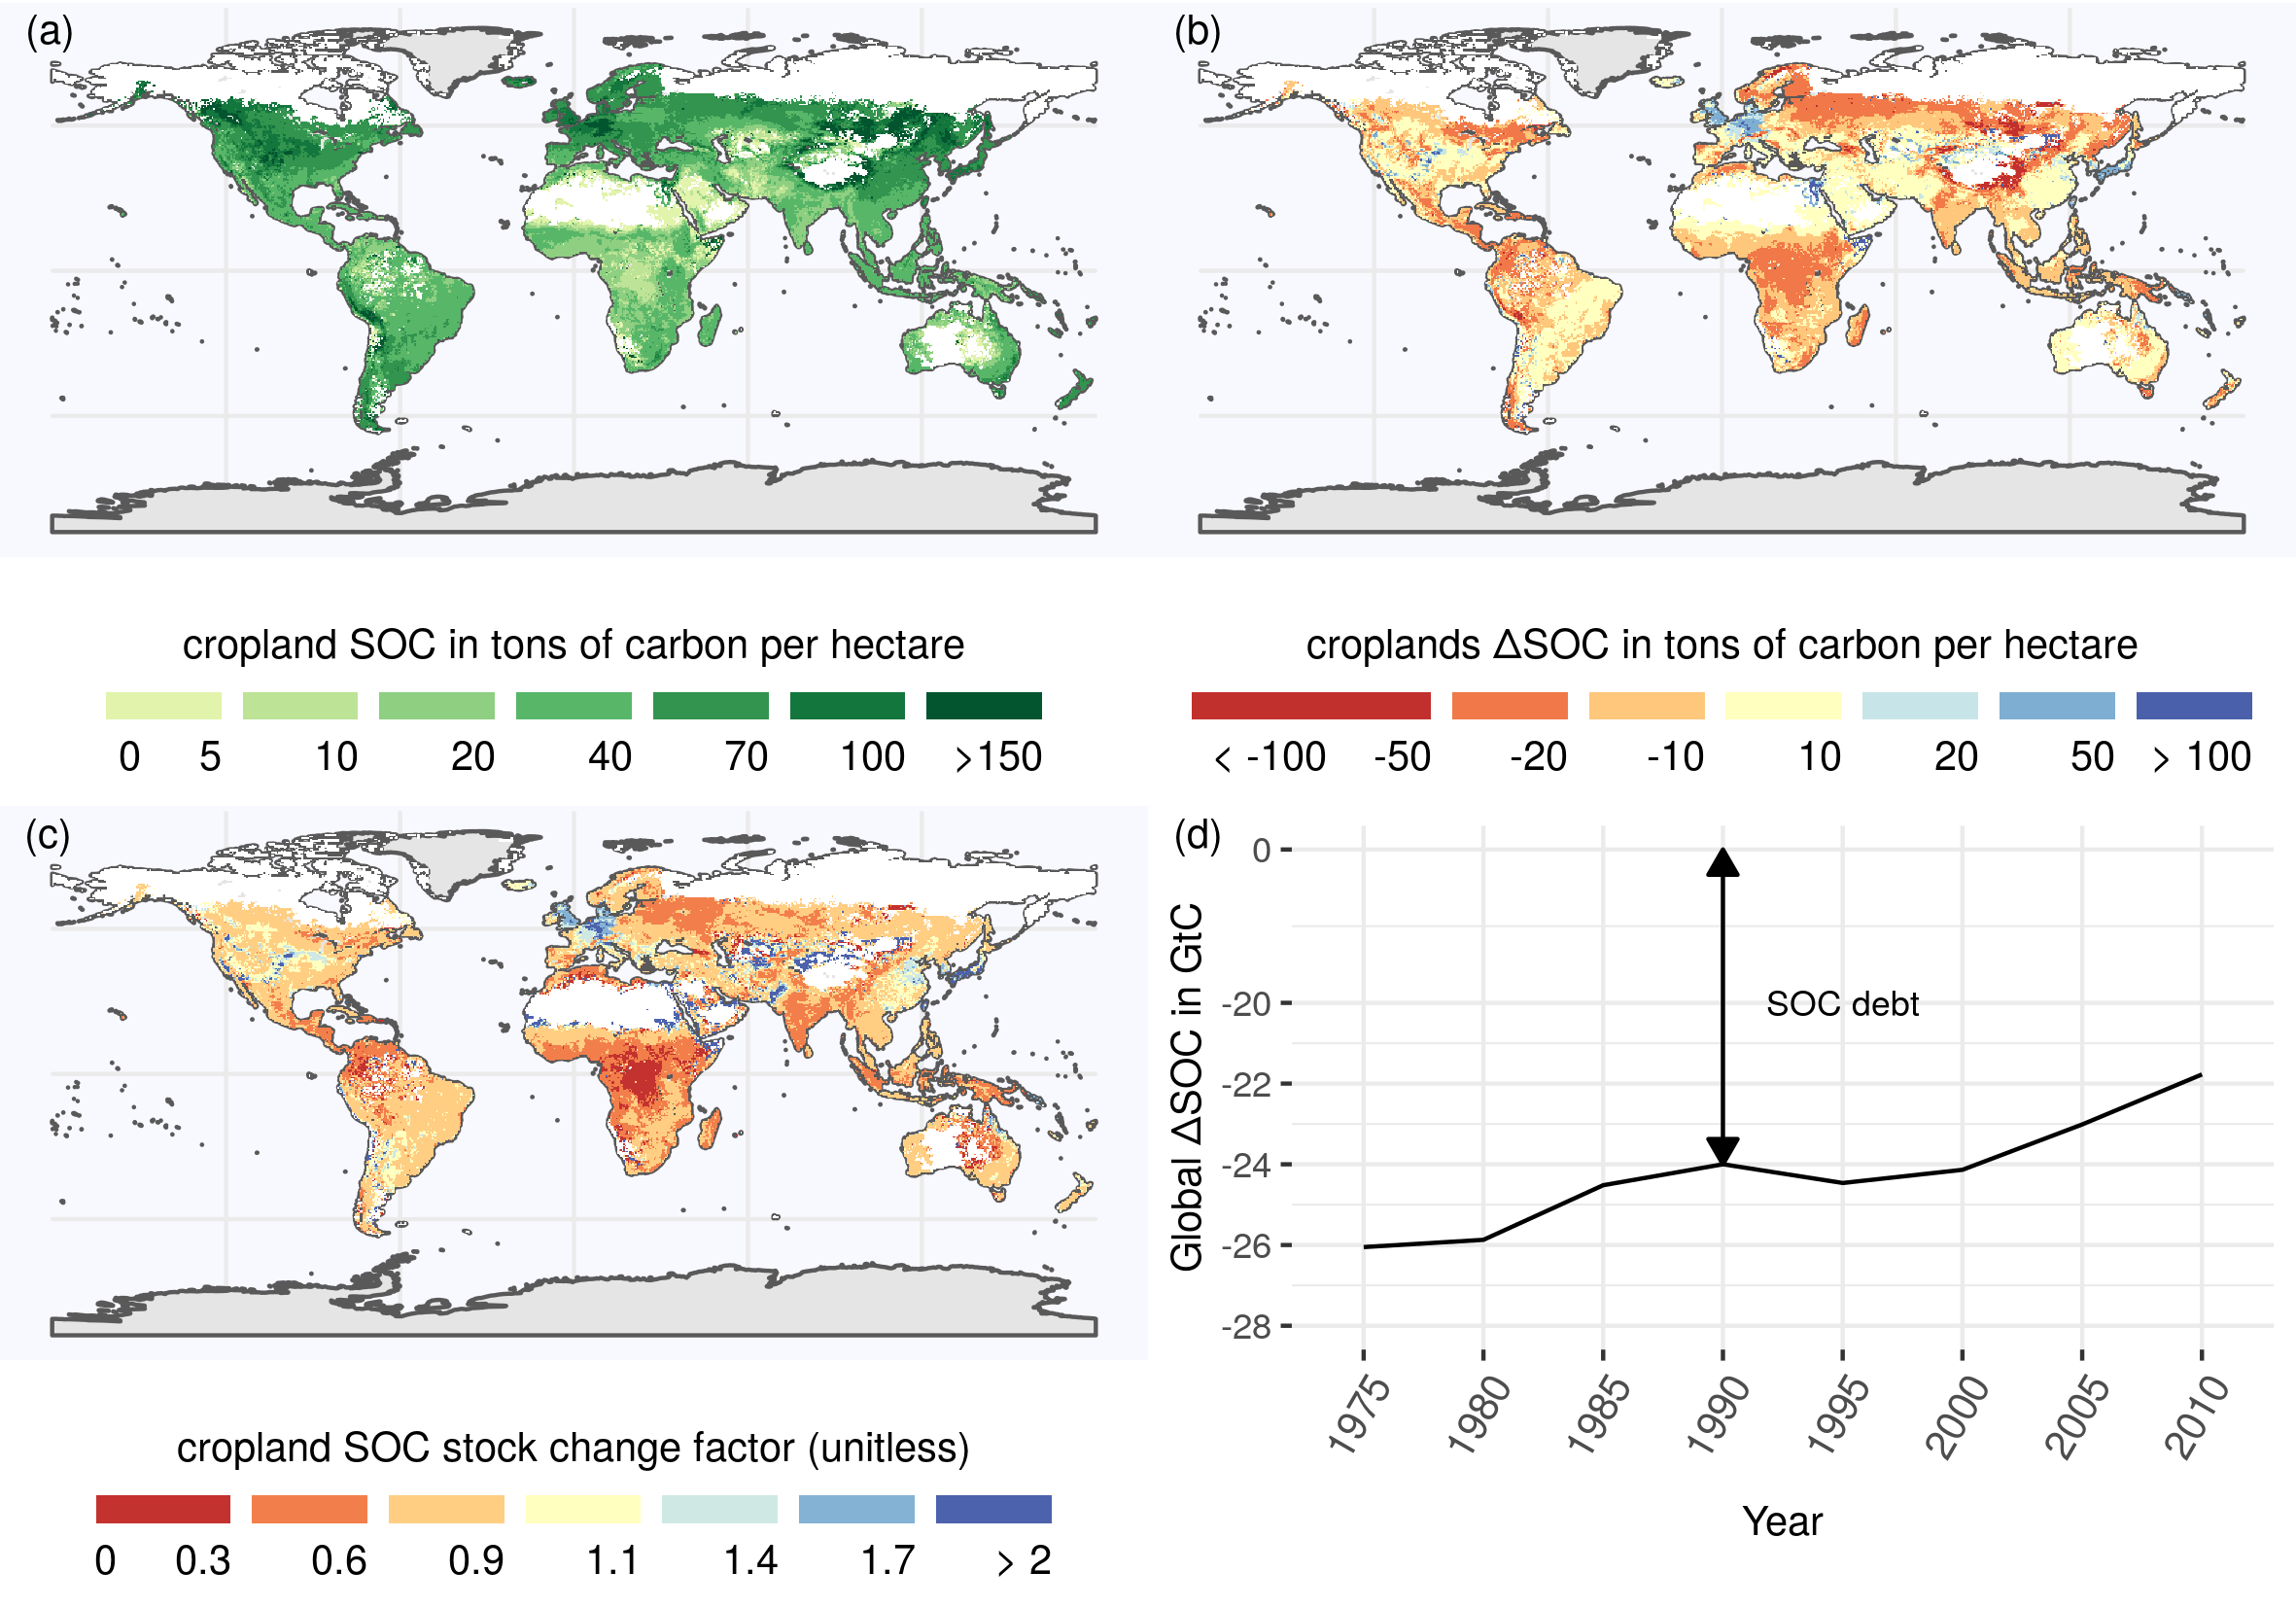
\includegraphics[width=18cm]{../ResultNotebooks/Output/Images/4panelfigure} \caption{(a): Distribution of total global SOC stocks for the first 30 cm on cropland:  Carbon stocks are large in high yielding areas. (b)+(c): Absolute (b) and relative (c) SOC stocks changes compared to a potential natural state identify different hotspots of SOC dynamics. Whereas absolute losses $\Delta SOC$ are often highest in temperate dry regions, relative losses $F^\mathrm{SCF}$ are often larger in tropical moist areas. (d): $\Delta SOC$ between SOC under historic land use and potential natural vegetation is decreasing over time, meaning net SOC gains on global croplands over the the period 1975--2010. }\label{fig:SOCmaps}
\end{figure}

In Fig. \ref{fig:SOCmaps}(a) we provide the first world map of SOC stocks for the first 30 cm on croplands considering historic management data at the global scale for the year 2010. Values ranging between well over \(100\unit{t ha^{-1}}\) in northern temperate croplands to less than \(5\unit{t ha^{-1}}\) for arid and semiarid croplands.
Our spatially explicit results show hotspots of SOC losses and gains compared to SOC under potential natural vegetation in two complementary ways:
1. Absolute SOC changes \(\Delta SOC\) (see Fig. \ref{fig:SOCmaps}(b)) indicate areas with high importance for the global SOC losses. They might be driven by large relative changes (e.g.~in Central Africa) or by a high natural stock, from which even small relative deviations could lead to substantial absolute losses (e.g.~North-East Asia). In contrast, large net gains of SOC occur primarily in developed countries of the Global North according to our results.
2. Relative SOC changes measured as stock changes factors \(F^{SCF}\) (see Fig. \ref{fig:SOCmaps}(c)) are a helpful metric to analyze the impact of human cropping activities. They indicate areas with large differences in carbon inflows or SOC decay compared to natural vegetation, that may hold potential to be overcome due to improved agricultural practices. Large parts of tropical croplands seem to suffer from low stock changes factors, meaning high relative SOC losses and maybe indicating SOC degradation. Conversely, not only temperate croplands of Central Europe, Japan and western areas of the USA have high stock change factors, but irrigated croplands at the border to dry, unsuitable areas worldwide as well.

The global SOC debt has decreased by about 15\% in the period between 1975 and 2010 to \(22\unit{GtC}\) (Fig. \ref{fig:SOCmaps}(d)). This corresponds to a sequestration rate of \(0.11\unit{GtC yr^{-1}}\). Considering our estimate of the global SOC stock of around \(660\unit{GtC}\) in 1975, global SOC increased by 0.2 per 1000 per year for the period between 1975--2010.

\hypertarget{carbon-flows-in-the-agricultural-system}{%
\subsection{Carbon flows in the agricultural system}\label{carbon-flows-in-the-agricultural-system}}

\begin{figure}[h]
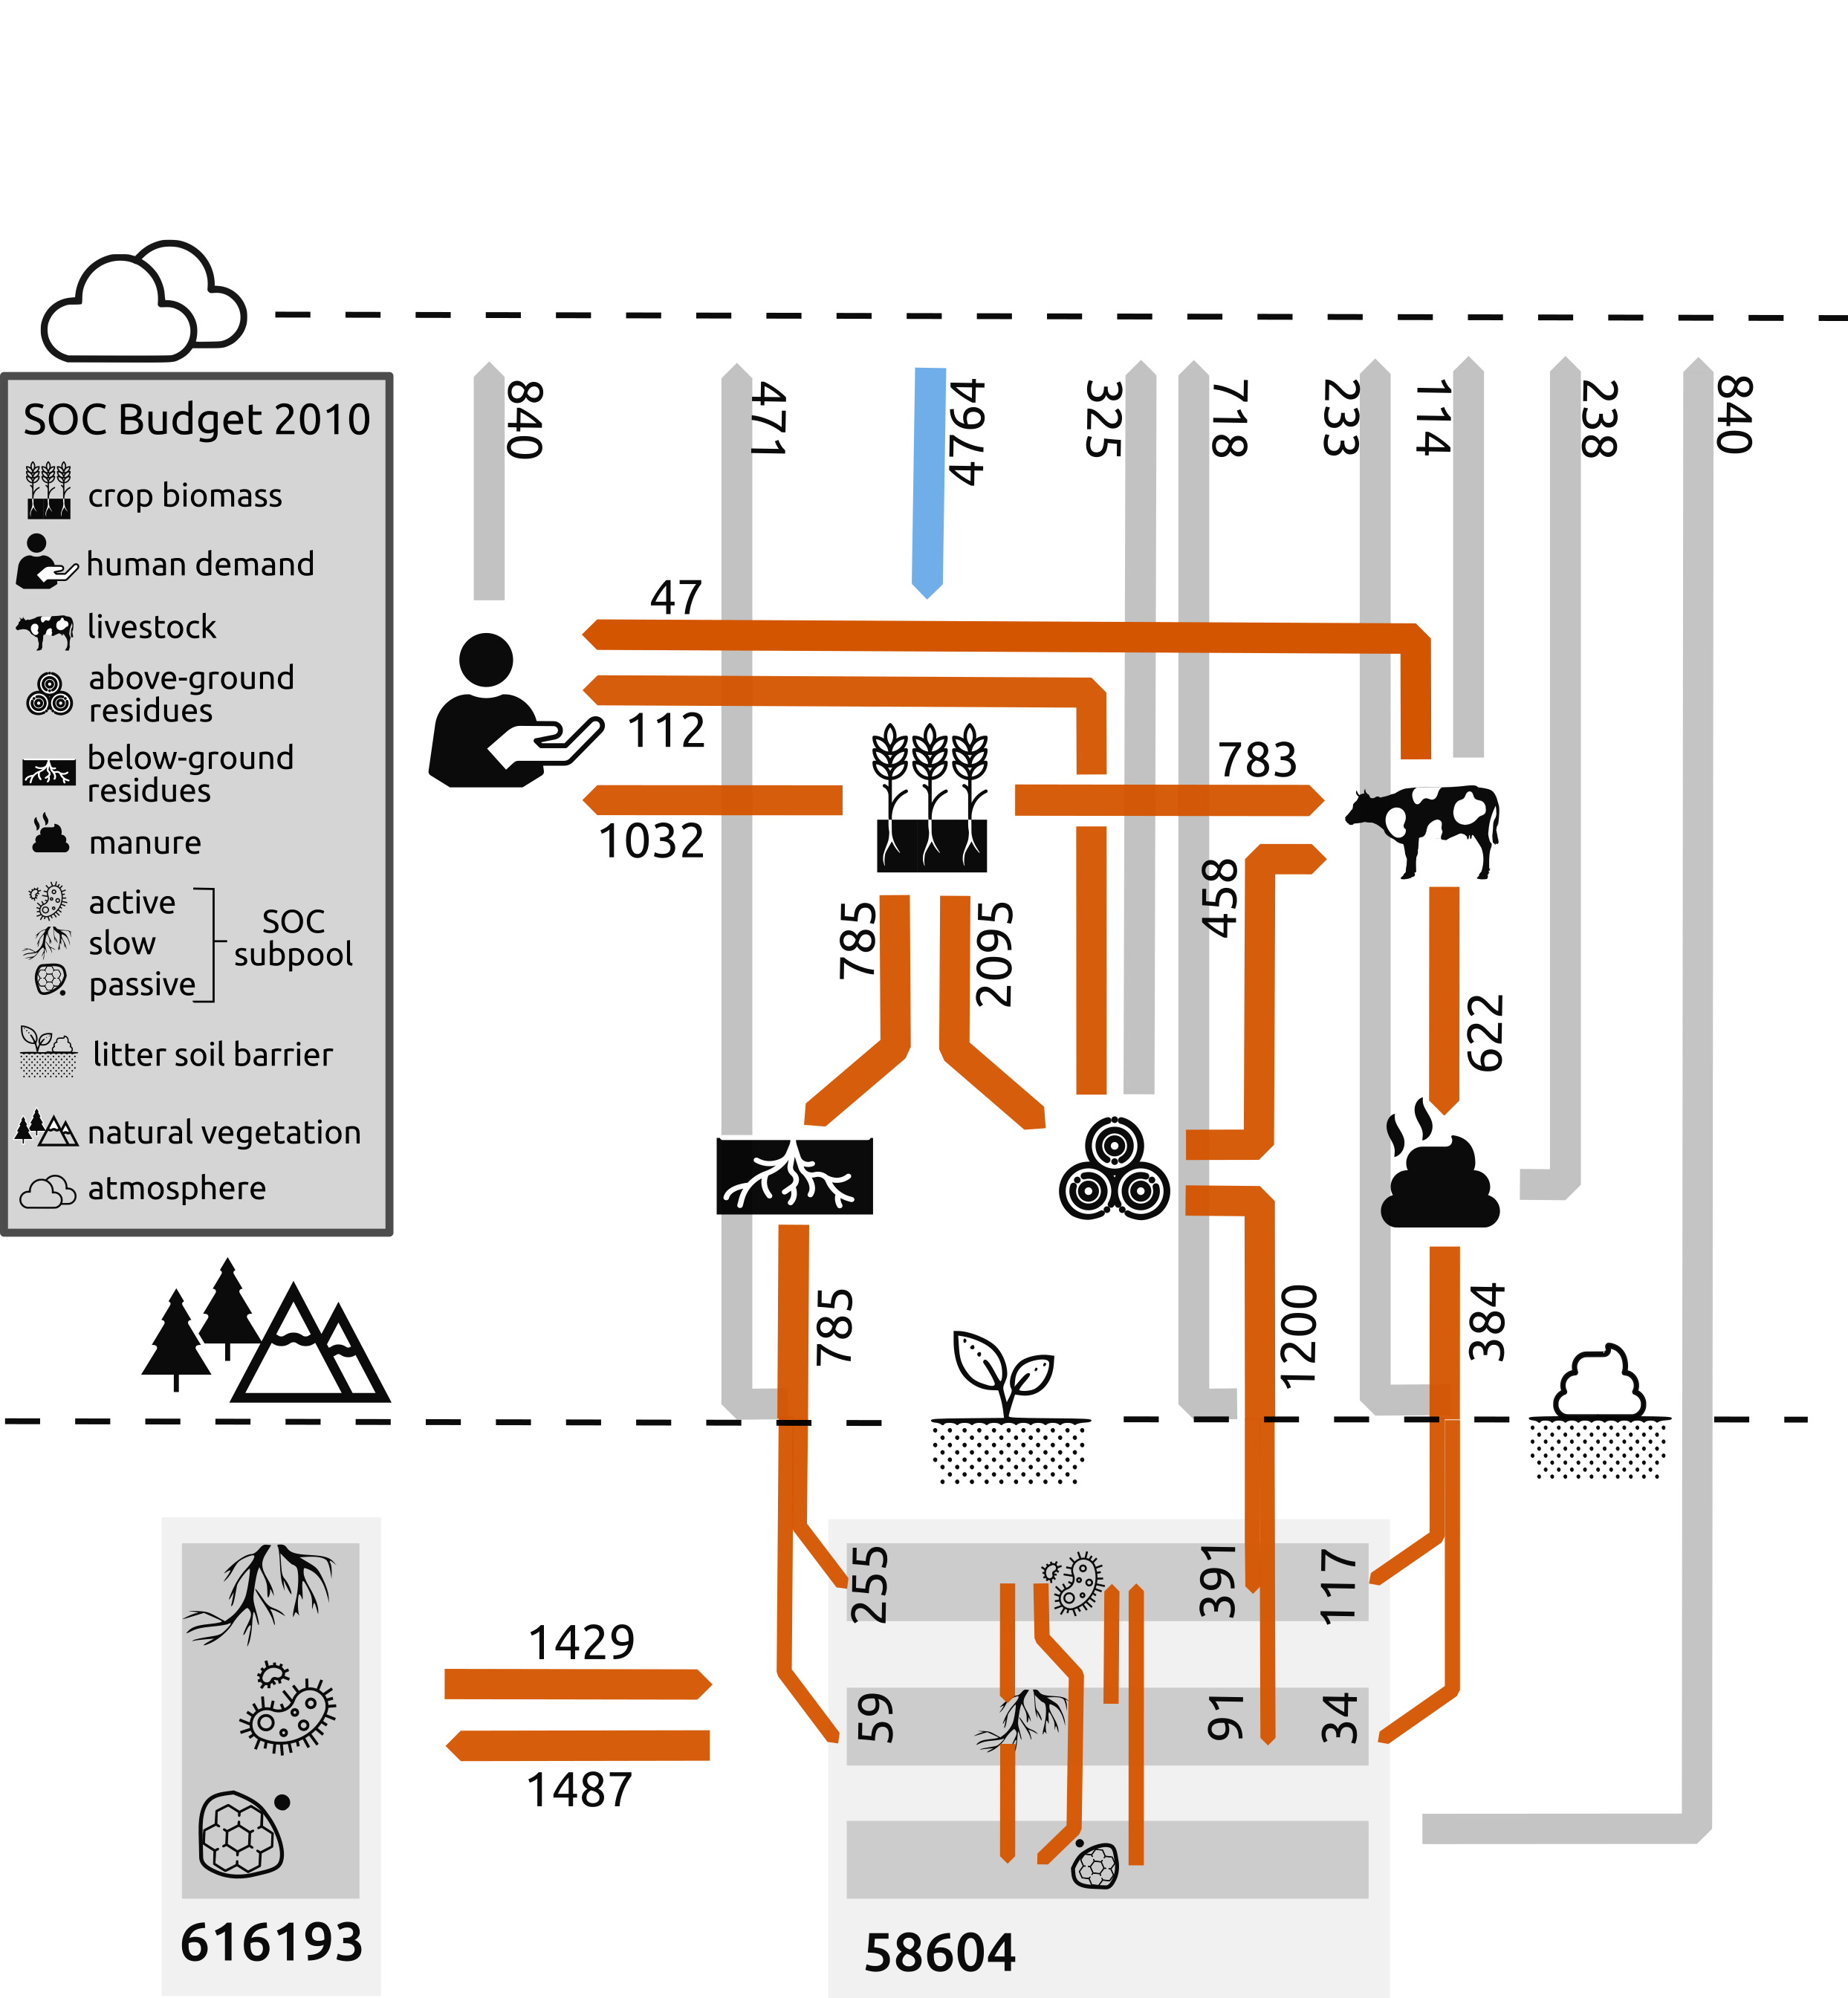
\includegraphics[width=16cm]{../ResultNotebooks/Output/Images/CarbonBudget} \caption{Global carbon flows within the agricultural system for the year 2010 (in MtC): Carbon is first photosynthesise by crop plants and than used depending on the plant part by humans for feed of livestock and various other usages subsumed under human demand. After accounting for losses within the agricultural system three major C inputs are applied to croplands: manure, above- and below-ground residues. Large parts of C, however, get mineralized on field before entering the soil. Additionally, C is transferred to and from agricultural soils via land-use change to and from natural vegetation. Finally, SOC gets mineralized and flows back into the atmosphere.}\label{fig:FlowFig}
\end{figure}

C is sequestered from the atmosphere via plant growth and allocated to three different plant parts (harvest organ, above- and below-ground residues). Whereas harvested organs as well as above ground-residues are taken (partially) from the field to be used for other purposes, below-ground residues (785 MtC in 2010) are directly returned to the field. We split up usage for crop biomass into feed usage and aggregate all other usage types (e.g.~like food, bioenergy and material) into a human demand category. Livestock feed demand for crop harvest and above-ground residues of 1141 MtC is almost equal to the human demand of 1144 MtC. Whereas large parts of feed intake are recycled to the soils via manure (C input from manure at 384 MtC), we assume the carbon demanded from humans (ending up as e.g.~compost, night soil and sewage) is not recycled to soils. Besides manure C and below-ground residues, above-ground residues form the largest C input to the soil with 1200 MtC returned to the field in 2010. However, around 60\% of C decomposes before its integrated into soils at the the litter-soil barrier. Due to the different C composition, proportional more C enters the slow pool from manure compared to crop residue. According to our model results, land-use change dynamics led to a C transfer from cropland to natural vegetation of 58 MtC in 2010. 4764 MtC sequestered by crop plants face 3897 MtC released within the agricultural system. Accounting for SOC transfer, SOC increase under cropland is around 809 MtC.

\hypertarget{agricultural-management-effects-on-soc-debt}{%
\subsection{Agricultural management effects on SOC debt}\label{agricultural-management-effects-on-soc-debt}}

\begin{figure}[h]
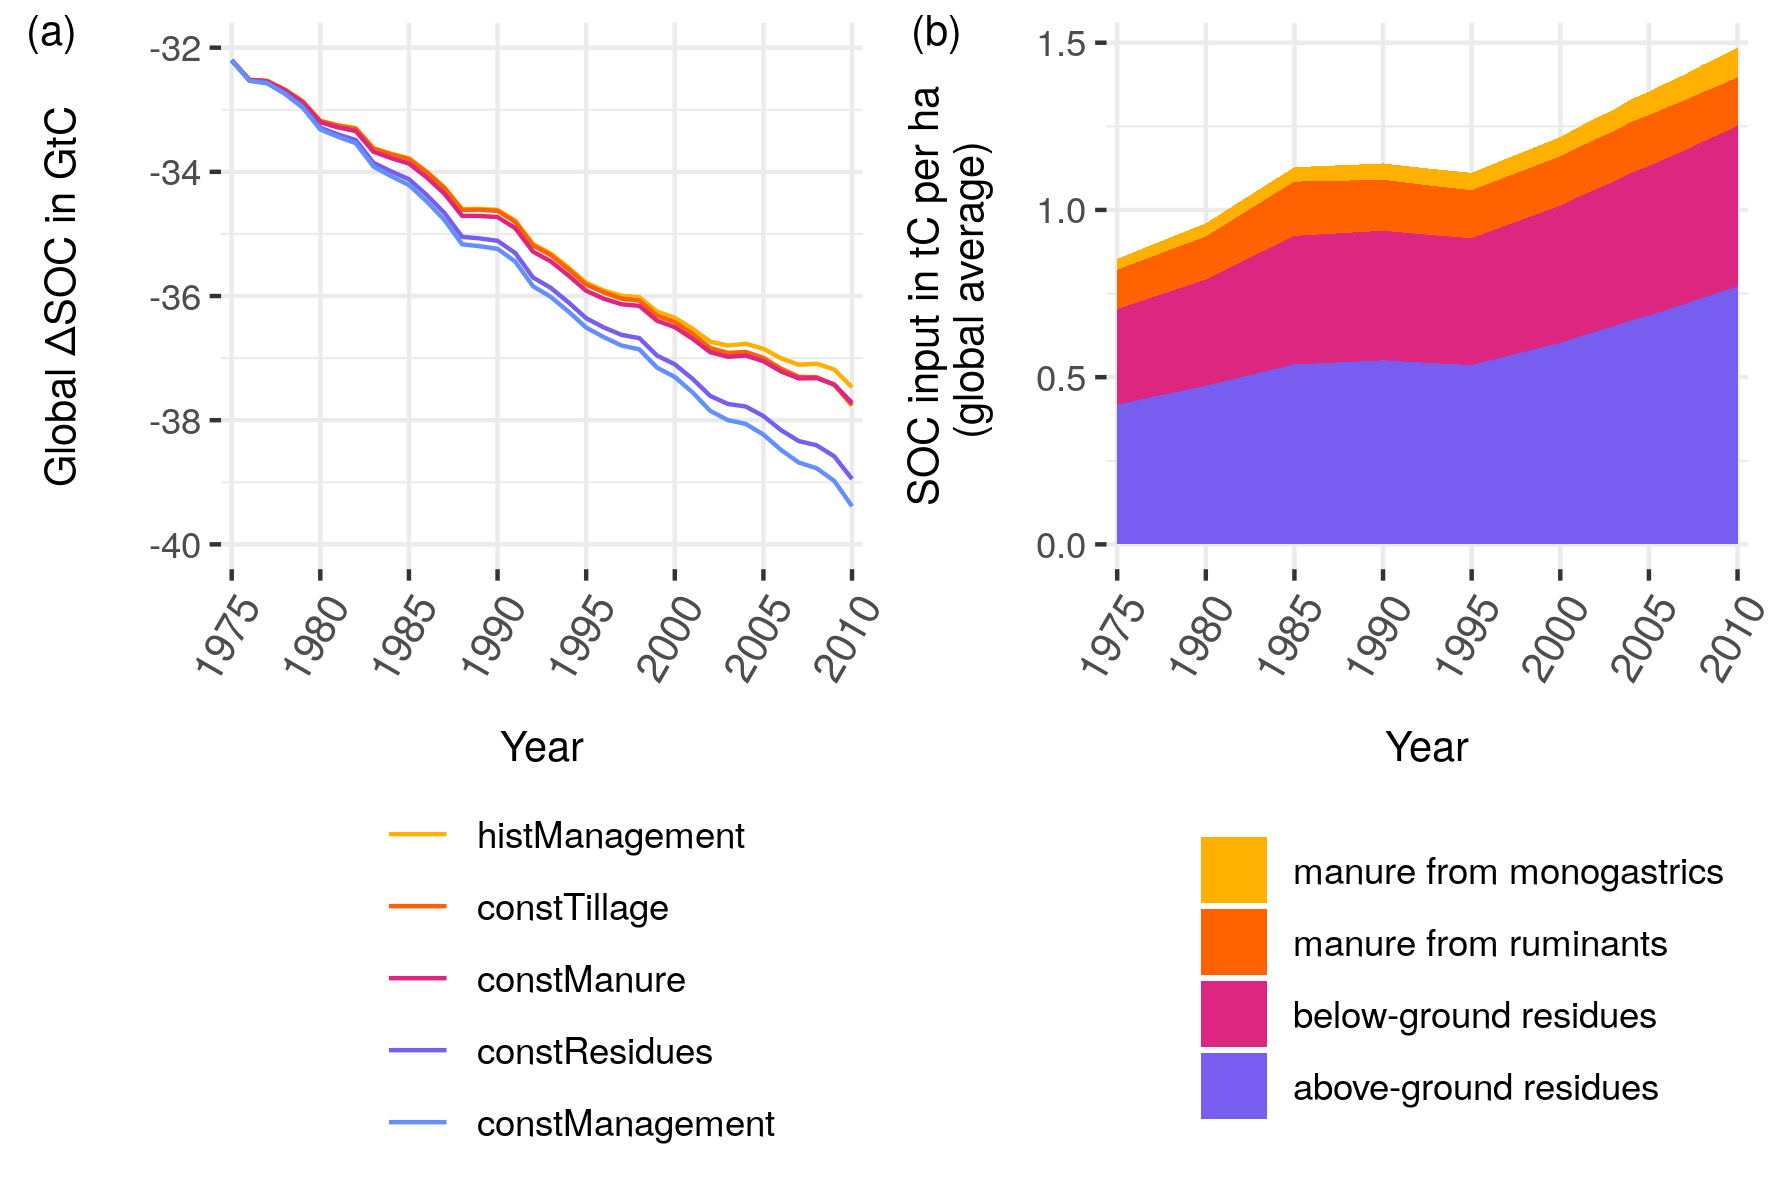
\includegraphics[width=14cm]{../ResultNotebooks/Output/Images/scenario_horiz} \caption{(a) Global $\Delta SOC$ in GtC for different management scenarios: The stylized scenarios devate from historic argicultural management by holding effects of carbon inflows from residues (constResidues), manure (constManure) constant or neglecting adoption of no-tillage practices (constTillage). ConstManagement combines all three modifications. Note that $\Delta SOC$ is defined as the difference of SOC under land-use compared to a natural vegetation state. Figure (b) shows the carbon inflows from crop residue and manure, underlining the strong impact of residues for SOC stock and SOC stock changes.}\label{fig:SOCscen}
\end{figure}

We analyze the relative impact of individual management aspects by comparing the actual historic management scenario with counterfactual scenarios where individual management aspects are kept static at the 1975 values (Figure \ref{fig:SOCscen}(a)). Without changes in management regimes, the global \(\Delta SOC\) on cropland would be increasing at a rate of \(0.1\unit{GtC yr^{-1}}\). As shown by the constResidue scenario, changes in residue return rates dominate the management effects. Without the historic increase in residue returning, the global \(\Delta SOC\) would still increase at a rate of \(0.06\unit{GtC yr^{-1}}\). Both the constManure and constTillage scenarios show only small deviations from the historic values (sequestration rate of \(0.09\unit{GtC yr^{-1}}\) for both). The effect of no-tillage has been particuarly strong since the 1990s.
The strong impact of almost doubling C inputs from crop residue biomass over a period of 35 years on agricultural SOC stocks is shown in Fig. \ref{fig:SOCscen}(b).

\begin{figure}[h]
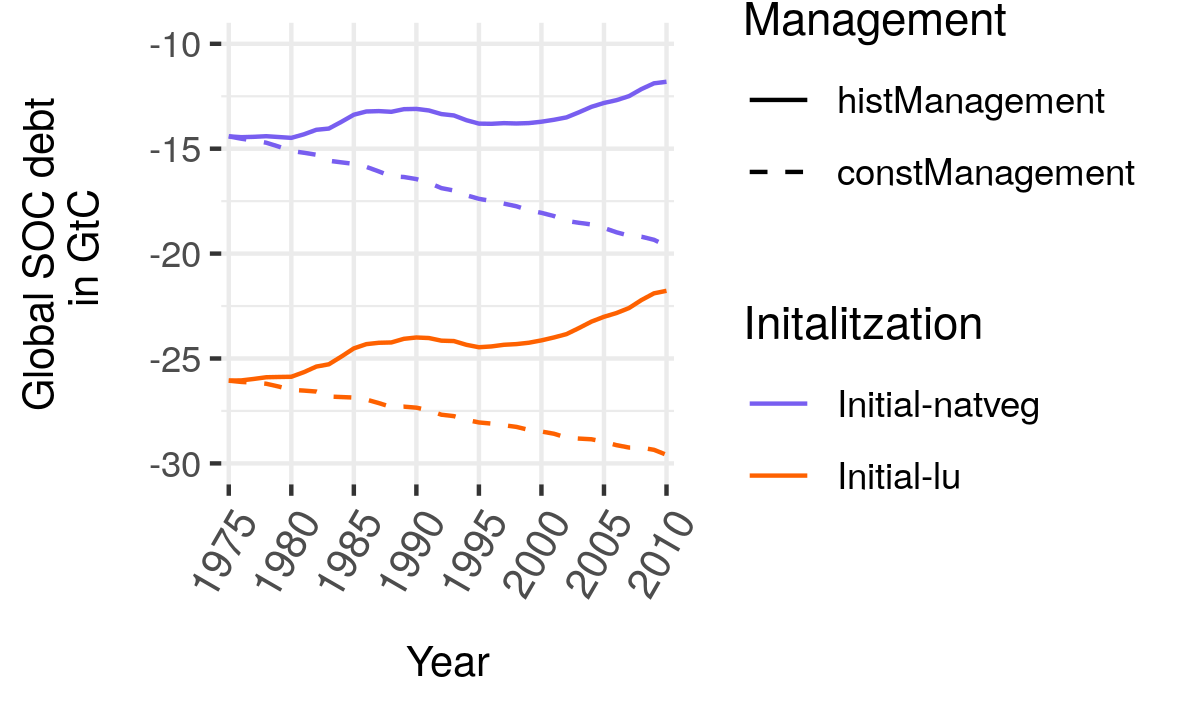
\includegraphics[width=10cm]{../ResultNotebooks/Output/Images/scenario_init} \caption{Global $\Delta SOC$ for different SOC initialization choices in the start year 1901: Starting the spin-up phase with natural steady-state SOC under vegetation without any human cropping activities (Initial-natveg) lead to a smaller $\Delta SOC$ in 1975 and a less steeper increase till 2010, as compared to initialzing with steady-state SOC stocks under historic land-use.}\label{fig:SOCinit}
\end{figure}

Our sensitivity analysis shows that the management impact is robust to the initialization of SOC stocks at the beginning of the spin-up phase (Fig. \ref{fig:SOCinit}). The Initial-natveg scenario initializes the start year with the steady-state SOC under potential natural vegetation for all land-use types, compared to the default assumption (Initial-lu), which assumes landuse-type specific steady-state SOC stocks in 1901. The \(\Delta SOC\) estimation almost halves (from \textasciitilde26 GtC to \textasciitilde14 GtC), as does the decrease in \(\Delta SOC\) for the period of 1975--2010 (from \textasciitilde4 GtC to \textasciitilde2.5 GtC) for the Inital-natveg scenario.

Global SOC stocks range between 645--700 GtC for different parameterization of the natural litterfall, whereas \(\Delta SOC\) vary 19-24 GtC for the year 2010 (see Fig. \ref{fig:SOClitter}. The increase of \(\Delta SOC\) during the period of 1975--2010 is independent of the parameterization choice at \textasciitilde4 GtC.

\newpage

\hypertarget{discussion}{%
\section{Discussion}\label{discussion}}

This study shows that spatially explicit and time-variant historic agricultural management data considerably alter estimates of the states and trends of SOC compared to the often used constant management assumptions. This result remains robust to variations of central model parameters and variations in the initialization of SOC stocks. While land cover change has depleted SOC stocks and increased the SOC debt, our analysis points out that the high increases in agricultural productivity may have even led to a net reduction of the SOC debt since 1975.

\hypertarget{soc-debt-and-soc-drivers-in-literature}{%
\subsection{SOC debt and SOC drivers in literature}\label{soc-debt-and-soc-drivers-in-literature}}

The evaluation of SOC stock gains and losses is complex and has several dimensions as climatic and anthropogenic effects overlap. If defining the SOC debt of 1975 as the baseline, and measuring land-use emissions on croplands as the difference between a potential natural state and the state under human interventions \citep[see][]{pugh_simulated_2015}, global croplands have acted as a carbon sink since 1975 according to our study. However, annual C sequesteration rates of 0.2 per 1000 are well below the promoted 4 per 1000 \citep{minasny_soil_2017}, indicating that productivity gains on historic levels alone are not enough to meet ambitious climate targets.

According to Sanderman et al.~\citeyearpar{sanderman_soil_2017}, the SOC debt since the beginning of human cropping activities has been at around 37 GtC for the first 30 cm of the soil with half of it attributed to SOC depletion on grasslands. Our estimate of 22 GtC in 2010 for cropland debt is higher as Sanderman et al.~\citeyearpar{sanderman_soil_2017} estimations. However, there are large uncertainties in modeling SOC at the global scale, and Sanderman et al.~\citeyearpar{sanderman_soil_2017} pointed out that their results might be conservatively low compared to experimental results. This suggests that our results are within a plausible range.

Furthermore, Sanderman et al.~\citeyearpar{sanderman_soil_2017} modeled historic trends based on agricultural land expansion without considering SOC variations due to time-variant agricultural management. Pugh et al.~\citeyearpar{pugh_simulated_2015} considered management effects like tillage and residue returning in a static way, but neither changes over time nor alignment to observed historic data like yield-levels or no-tillage areas were taken into account. Their study moreover concludes that crop productivity-gains (increasing yield levels by 18\% in their simulations) do not lead to a~substantial decline in SOC debt (less than 1\% change). Historic productivity increases were, however, notably larger. Despite large spatial heterogeneity aggregate yield increase rates are often estimated to be well above 50\% \citep{pellegrini_crop_2018, ray_recent_2012, rudel_agricultural_2009}.

Our study for the first time uses a dynamic management dataset as driver for SOC dynamics. We show that the moderate global cropland expansion of around 11\% between 1974 and 2010 and the resulting depletion of SOC stocks in converted cropland has been outweighed by improvements in agricultural productivity and practices. This is in contrast to Pugh et al.~\citeyearpar{pugh_simulated_2015} findings of only small effects due to improved practices.

Looking on historic cropland intensification rates of above 50\% \citep{rudel_agricultural_2009}, a large fraction of increased C input from residue biomass is attributed to productivity improvements.

\hypertarget{limitations-and-uncertainties}{%
\subsection{Limitations and uncertainties}\label{limitations-and-uncertainties}}

Modeling management effects at the global scale comes with parametric and structural uncertainties. High SOC gains in the first 30 cm of the soil compared to natural vegetation in e.g.~the temperate croplands of Central Europe and the United Kingdom indicate suspiciously high estimates of SOC inputs. As pointed out by Keel et al.~\citeyearpar{keel_large_2017} and Smith et al.~\citeyearpar{smith_how_2020}, carbon input calculations are highly sensitive to the choice of allometric functions determining below- and above-ground residue estimates from harvested quantities (see \ref{tab:c2dm} for coefficients used in this study). Keel et al.~\citeyearpar{keel_large_2017} question whether below ground residues might increase with a fixed root:shoot ratio rather than being independent of productivity gains. Moreover, the study pointed out that plant breeding shifts allometries, which might not be reflected in outdated data sources. While our study considers a dynamic harvest index with rising yields for several crops, we may still overestimate residue biomass in particular for below-ground biomass. However, looking on the evaluation of management effects (see Sect. \ref{sec:ipcccompare}), there is no general indication of overestimating stock change factors at least compared to IPCC default assumptions. Moreover, it is also likely that we are still missing carbon inputs to the soil from e.g.~cover- and inter-cropping practices.

Another uncertainty is connected with the initialization of SOC stocks in 1901, which is assumed to be in steady state considering the land-use pattern of 1901 and agricultural management data of 1965. As shown in Fig. \ref{fig:SOCinit} the SOC debt estimate almost halves (from \textasciitilde26 GtC to \textasciitilde14 GtC), and the SOC debt reduction is strongly reduced (from \textasciitilde4 GtC to \textasciitilde2.5 GtC), if considering initialization SOC stocks under undisturbed natural vegetation. Pugh et al.~\citeyearpar{pugh_simulated_2015} pointed out the importance of accounting for the land-use history, as many CO\textsubscript{2} emissions from agricultural soils are caused by historic land-use change (LUC) and the slow decline of SOC under cropland before it reaches a new equilibrium. Our results of the Initial-natveg scenario show that the qualitative finding of a reduction of SOC debt through improved agricultural management is robust to changing the initialisation of soil organic carbon, even though the level of SOC debt is sensitive to the initialization setting.

Generally, the limit to the first 30 cm of the soil profile follows the IPCC guidelines \citep{eggleston_ipcc_2006, calvo_buendia_ipcc_2019} and assumes that most of the SOC dynamic happens in the topsoil. In this regard several aspects are strongly simplified within our approach. Firstly, distribution of carbon inputs into different soil layers are neglected and all carbon inputs are allocated to the topsoil. This particularly overestimates SOC stocks in the first 30 cm of soil below deeper rooting vegetation, which is certainly the case for most of the woody natural vegetated areas. Secondly changes to the subsoil due to tillage are neglected. As Powlson et al.~\citeyearpar{powlson_limited_2014} have shown, the subsoil can be a game changer in evaluating total SOC losses or gains for no-tillage systems. No-tillage effects may seem larger than the actually are, if only focusing on the topsoil. SOC transfer to deeper soil layers under tillage, might enhance subsoil SOC compared to no-till practices. Thirdly, organic soils (like peat- and wetlands) and drained cropland areas are not explicitly considered and emissions from these cropland areas are thus likely substantially underestimated.

This study excludes not only peatland degradation, it also does not account for carbon displacement via leaching and erosion. However, as pointed out by Doetterl et al.~\citeyearpar{doetterl_erosion_2016}, the final fate of leached or eroded carbon is uncertain and might even offset LUC emissions \citep{wang_human-induced_2017}. Whereas for soil quality analysis SOC displacement might play an important role, in this budget approach focusing especially on the SOC debt, displaced but not emitted SOC can be treated as SOC that remains on the cropland.
Moreover, the exclusive focus on croplands ignores LUC emission on other land-use types such as pastures, rangelands and forestry. Human interventions have led to large changes in SOC stocks there as well \citep{sanderman_soil_2017, friedlingstein_global_2019}. This study does not intend to be a comprehensive LUC emission analysis and acknowledges that land-use changes comes with large overall emissions.

\hypertarget{sec:ipcccompare}{%
\subsection{Modeled management effect in line with default IPCC assumptions}\label{sec:ipcccompare}}

To validate our modeled SOC stocks and stock changes under management, we compare our results to default IPCC stock changes factors of 2006 \citep{eggleston_ipcc_2006} and their refinements in 2019 \citep{calvo_buendia_ipcc_2019}. Both estimates are based on measurement data for croplands (see Table \ref{tab:SCFglo}). To allow for comparison, we aggregate our stock change factors to the four IPCC climate zones (Fig. \ref{fig:CLIMzone}).

\begin{table}[ht]
\centering
\caption{$F^{\mathrm{SCF}}$ in comparison to IPCC Tier 1 default factors: Stock change factors are in good agreement with the default values of the IPCC in general. For the tropical regions the assumptions changed notablly from the guidelines in 2006 \citep{eggleston_ipcc_2006} to the update in 2019 \citep{calvo_buendia_ipcc_2019}. leaving our results in very good agreement with the old default assumptions. Default assumption are given under the assumption of medium input systems, which, considering the yield gap in mainly developing regions in the tropics, might be an overestimation and decrease $F^{\mathrm{SCF}}$ by additional 5-8 percent. Also modelled $F^{SOC}$ have increased for all climates over time.} 
\label{tab:SCFglo}
\begin{tabular}{rlllllll}
  \hline
 & Source & Input & Year & tropical moist & tropical dry & temperate dry & temperate moist \\ 
  \hline
1 & IPCC2006 & low & invariant & 0.44 & 0.55--0.61 & 0.74 & 0.66 \\ 
  2 & IPCC2006 & medium & invariant & 0.48 & 0.58--0.64 & 0.80 & 0.69 \\ 
  3 & IPCC2006 & high & invariant & 0.53 & 0.60--0.67 & 0.83 & 0.77 \\ 
  4 & IPCC2019 & low & invariant & 0.76 & 0.87 & 0.70--0.71 & 0.66--0.67 \\ 
  5 & IPCC2019 & medium & invariant & 0.83 & 0.92 & 0.76--0.77 & 0.69--0.70 \\ 
  6 & IPCC2019 & high & invariant & 0.92 & 0.96 & 0.79--0.80 & 0.77--0.78 \\ 
  7 & This Study & hist & 1990 & 0.57 & 0.61 & 0.78 & 0.76 \\ 
  8 & This Study & hist & 2010 & 0.64 & 0.68 & 0.83 & 0.83 \\ 
   \hline
\end{tabular}
\end{table}

Whereas our estimates are lower in the two tropical climate zones, temperate zone default factors are higher than Calvo Buendia et al.~\citeyearpar{calvo_buendia_ipcc_2019}. The tropical factors differ substantially between the IPCC guidelines in 2006 \citep{eggleston_ipcc_2006} and their refinement in 2019 \citep{calvo_buendia_ipcc_2019}, with our estimates within this range.
Taking the simplified assumption, that tropical soils might suffer from insufficient C input rates (low) due to yield gaps, whereas temperate soils in developed regions might be highly managed and fertilized (high), the difference vanishes partially. Our results still show especially in temperate dry regions --- the smallest region area-wise --- small deviations from natural SOC stocks. Considering the impact of irrigation and fertilization on carbon-poor dryland soils, even factors above 1 (see Fig. \ref{fig:SOCmaps}(c)) may be expected.

With regard to the time trend, our study shows the substantial impact of changing management factors on the development of stock change factors as also indicated by the time trend of the SOC debt.

\hypertarget{soc-stocks-in-line-with-literature}{%
\subsection{SOC stocks in line with literature}\label{soc-stocks-in-line-with-literature}}

The world's SOC stock and its changes are highly uncertain, which is seen in the wide range of global SOC stock estimates for the first 30 cm of the soil profile \citep{batjes_harmonized_2016, hengl_soilgrids250m_2017, fao_global_2018, schaphoff_lpjml4_2018-1} in Table \ref{fig:SOCglo}).

\begin{figure}[h]
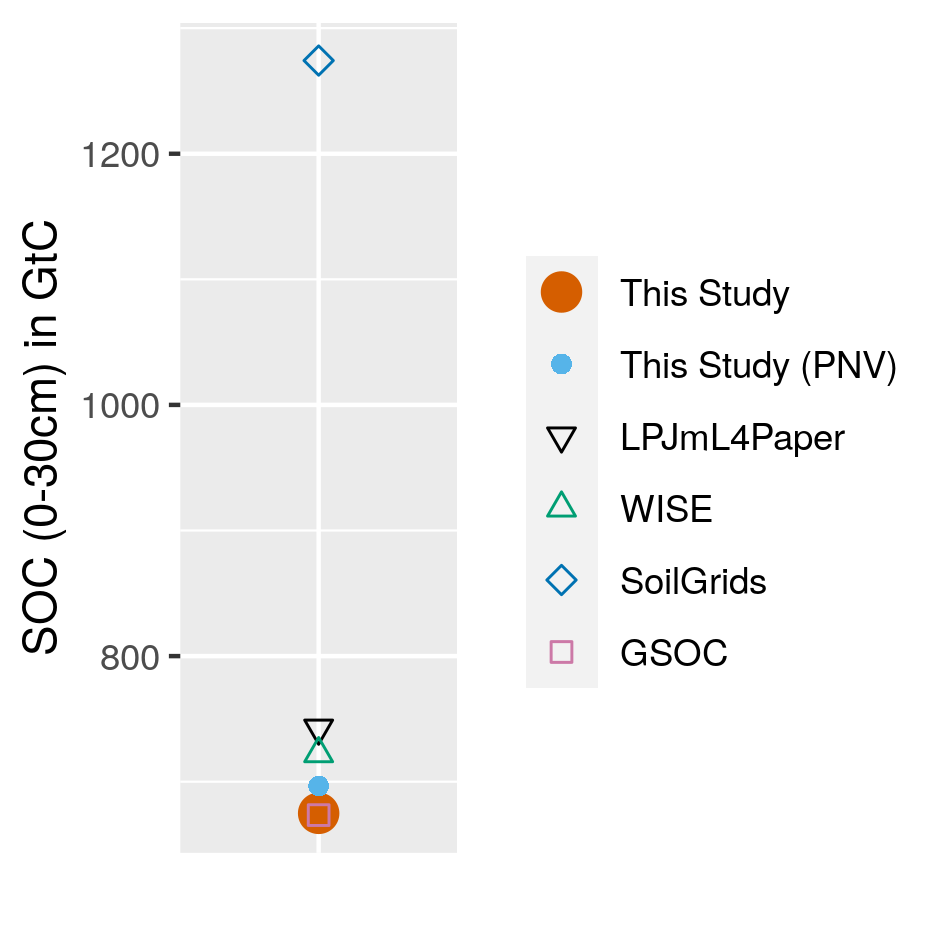
\includegraphics[width=8cm]{../ResultNotebooks/Output/Images/glo_comparisonfigure} \caption{Modeled as well as data based estimation for global SOC stock in GtC for the first 30 cm of soil aggregated over all land area: Note that SoilGrids, GSOC and WISE do not consider land-use as well as changes over time and rely on soil profile data gather over a long period of time. This makes it hard to pinpoint a specific year for these SOC estimations. In this context they will be compared to modeled data from LPJmL4 for potential natural vegetation and this study for the year 2010.}\label{fig:SOCglo}
\end{figure}

The global estimates of the total SOC stock from this study are on the lower end compared to other modeled results or data driven estimates. SoilGrids \citep{hengl_soilgrids250m_2017} especially stands out for their high estimation, whereas all other sources (including our study) are comparabely similar. Looking at regional results in Fig. \ref{fig:SOCreg}, our estimates turn out to be in good agreement for most of the world, with the largest deviations for boreal moist and tropical moist areas. To avoid that this bias influences our results, which originates from uncertainties in the representation of natural land, we focus on SOC changes on cropland. Pristine natural vegetated areas (like permafrost and rain forests) without human land management thus drop out in our calculation of SOC debt and stock change factors.

Additionally, our estimates for total SOC stocks of the world (as well as our SOC initialization) are dominated by the representation of natural vegetation, which are only estimated in a basic manner. For example, we do not differentiate the parameterization of nitrogen and lignin content of litterfall for woody and grass plant types. This renders carbon inputs and decay dynamics for natural litterfall rather uncertain. The absolute values of SOC stocks and debt from land-use change have to be interpreted with caution. As our default litter parameterization accounts for woody plant types, larger uncertainty in natural land SOC dynamics may arise especially in less forested areas.

We conducted a sensitivity analysis (Fig. \ref{fig:SOClitter}) based on various plant parameterizations from the Century model (see Sect. \ref{sec:scenlitterpnv}). This shows that the general trend of decreasing SOC debt of \textasciitilde4 GtC within the period of 1975--2010 is not altered under various estimates for natural SOC stocks.
\newpage

\conclusions

Our global SOC model is able to estimate spatially explicit SOC stocks, SOC debts and stock change factor considering agricultural management. It is --- to our knowledge --- the first study that quantifies the impact of time-variant and spatially explicit historic agricultural management on global SOC stocks.

Our results clearly demonstrate that agricultural management needs to be explicitly considered in global carbon assessments and models. That also implies that we need better monitoring of agricultural practices to create this data, but also better accessibility of existing data. Our data-set and the MADRaT package \citep{dietrich_madrat_2020} constitute a starting point for building comprehensive data sets on agricultural management aspects.

Our study again highlights that the expansion of croplands is still a major source of CO\textsubscript{2} emissions --- not only by the removal of vegetation, but also by a slow depletion of soils. Our estimates indicate a SOC debt of 22 GtC in 2010, and every additional deforestation adds to this debt.

However, our results also indicate that the changes in cropland management have led to increased SOC stocks in global cropland soils as a continuous trend since 1975. Even more, this trend of improved management on existing croplands more than overcompensates the depletion of SOC stocks on newly converted soils. The finding of this recovery of cropland SOC stocks challenges the assumption that cropland soils are a CO\textsubscript{2} source. Only under the assumption that cropland management is static over time, as typically assumed in other studies on cropland SOC stocks, we can reproduce their finding that cropland soils are a source of CO\textsubscript{2}. The estimated increase in cropland SOC is therefore caused by changing agricultural management, with the largest contribution stemming from increased carbon inputs to soils from crop residues.

Continuing the historical development, a further closure of the yield gaps may be beneficial to SOC stocks. Forest protection schemes for climate change mitigation would not only reduce SOC losses on newly converted land, they would likely also require further productivity improvements in existing croplands to meet crop demand \citep{popp_land-use_2014-1} --- and thereby usually further reduce the SOC debt on croplands.

While further crop productivity gains lead to co-benefits for SOC stocks, they are likely not enough to help meeting ambitious climate mitigation targets. Our findings on sequestration rates are still more than an order of magnitude lower than promoted by the 4 per 1000 initiative.

Yet, there is ample potential for further improved SOC management. As shown in Fig. \ref{fig:FlowFig}, approximately one fifth of total annual C sequestration by crops is lost through soils (0.8 GtC per year). Large losses in fact occur at the end of the food supply chain (1.2 GtC year), and at the litter soil barrier (1.4 GtC). Improved management could include, firstly, a circular flow from the food supply chain back to soils. Waste composting or excreta recycling could represent a major additional N input to cropland soils \citep{brenzinger_organic_2018}. Secondly, soil carbon sequestration techniques \citep{smith_soil_2016}, deep ploughing \citep{alcantara_deep_2016} or the transformation of c inputs to more recalcitrant biochar \citep{woolf_sustainable_2010} may transfer larger parts of the biomass at the litter soil barrier into permanent soil pools. Thirdly, reducing the share of residue burning and improved manure recycling could further increase C inputs. Finally, other carbon-accumulating practices, such as the cultivation of cover crops \citep{poeplau_carbon_2015} and agroforestry \citep{lorenz_soil_2014} could increase total C sequestration on croplands.




\codedataavailability{We compile calculations as open-source R packages available at github.com/pik-piam/mrcommons \citep{bodirsky_mrcommons_2020} for the management related functions, github.com/pik-piam/mrsoil \citep{karstens_mrsoil_2020} for soil dynamic related functions and github.com/pik-piam/mrvalidation \citep{bodirsky_mrvalidation_2020} for validation data. All libraries are based on the MADRaT package at github.com/pik-piam/madrat \citep{dietrich_madrat_2020}, a framework which aims to improve reproducibility and transparency in data processing. Model results including C input data are accessable under \url{https://doi.org/10.5281/zenodo.4320663} \citep{karstens_model_2020}. Software code for paper and result prepartion can be found under www.github.com/k4rst3ns/historicalsocmanegement.} %% use this section when having data sets and software code available



%%%%%%%%%%%%%%%%%%%%%%%%%%%%%%%%%%%%%%%%%%
%% optional

%%%%%%%%%%%%%%%%%%%%%%%%%%%%%%%%%%%%%%%%%%
\appendix
\section{Figures and tables in appendices}

\subsection{Methods}

\begin{figure}[h]
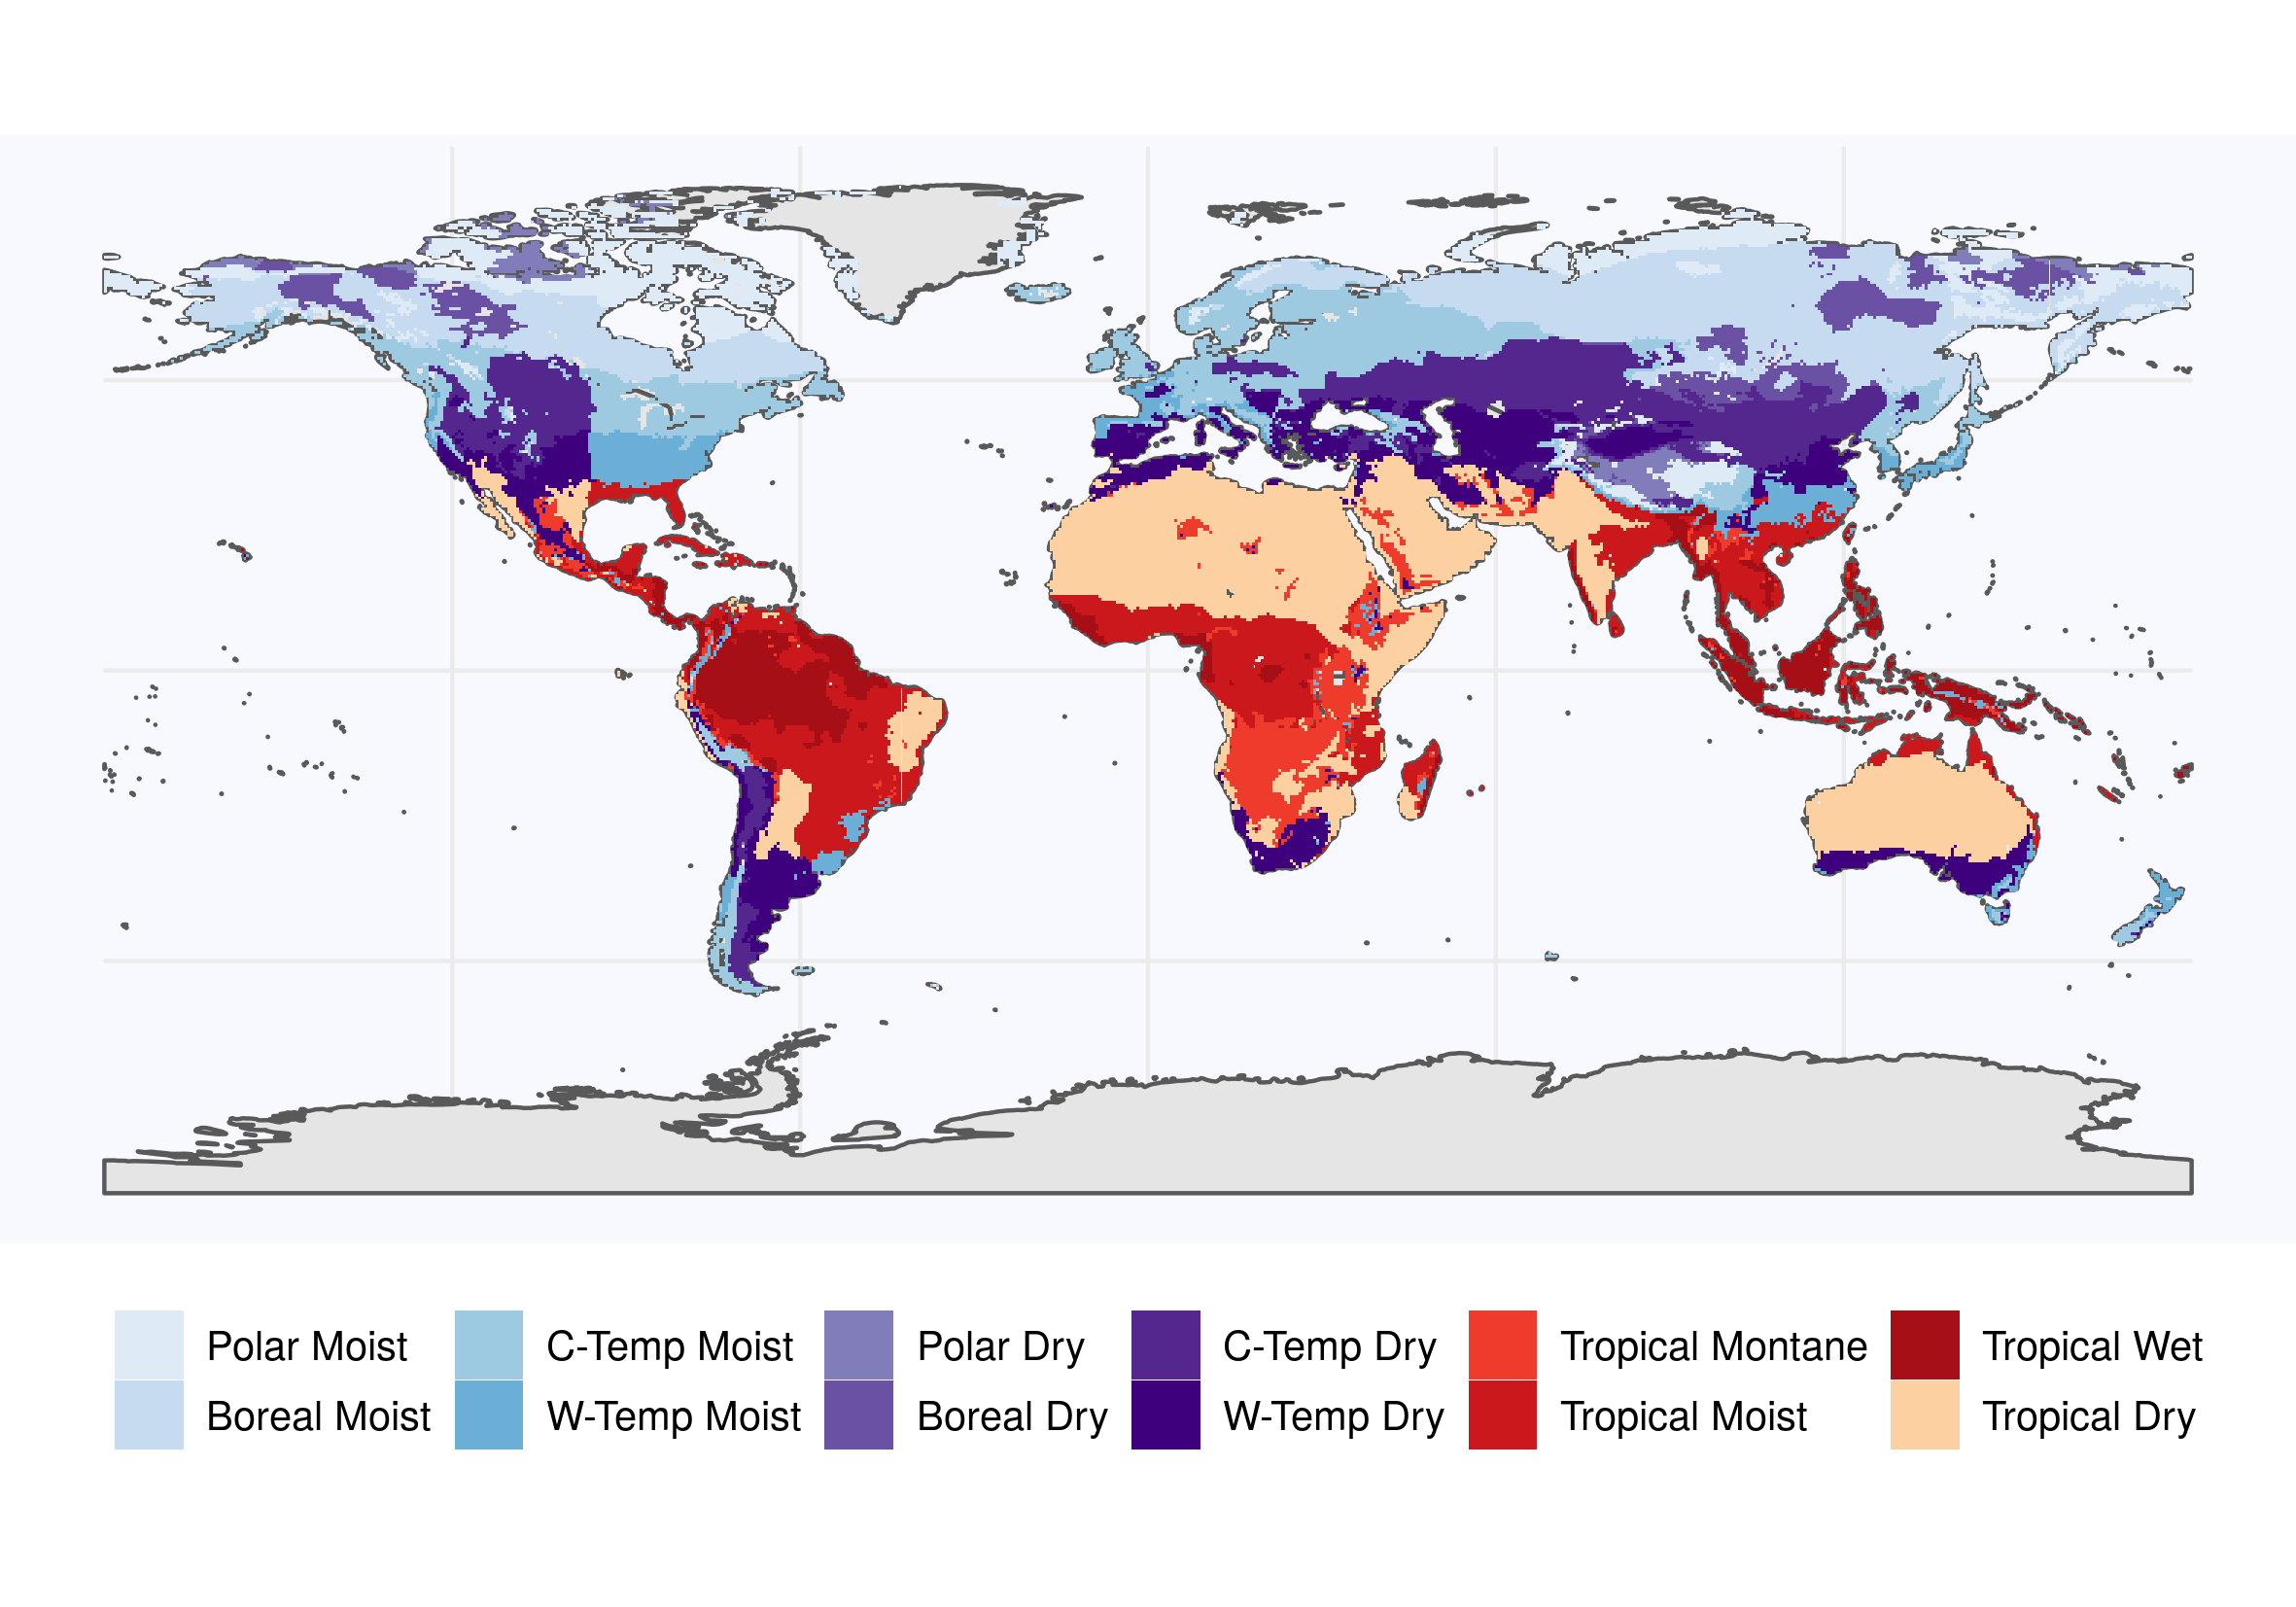
\includegraphics[width=13cm]{../ResultNotebooks/Output/Images/climatezones} 
\caption{Climate zone map adpated from IPCC: The climate zone classification is based on the classification scheme of the IPCC guidelines \citep{eggleston_ipcc_2006} and has been reimplented by \citet{carre_background_2010}, which is the source of this data. Note that the reduced set, used for the comparison of stock change factors is included in the color code with temperate moist in light blue, temperate dry in dark violett, tropical moist in red and tropical dry in orange.}
\label{fig:CLIMzone}
\end{figure}

\begin{sidewaystable*}[htbp]
\caption{Parameterization of harvested organs and their corresponding residues parts as well as allometric coefficients: This table is mainly based on \citet{bodirsky_n2o_2012} together with simple carbon to dry matter assumptions. Allometric coefficients are used as descriped in \citet{eggleston_ipcc_2006} with HI\textsuperscript{prod} being slope\textsubscript{(T)}, HI\textsuperscript{area} intercept\textsubscript{(T)} and RS R\textsubscript{BG-BIO}.
}
\begin{tabular}{lllllllllllll}
\tophline

         &                                 & \multicolumn{3}{l}{Harvested Organs} & \multicolumn{3}{l}{Above-ground Residues} & \multicolumn{2}{l}{Below-ground Residues} & \multicolumn{3}{l}{Allometric coefficients}                \\
Crop code  & Crop Type                       & nr/dm       & wm/dm      & c/dm      & nr/dm         & wm/dm        & c/dm       & nr/dm                & c/dm               & HI\textsuperscript{area} & HI\textsuperscript{prod} & RS   \\
 \middlehline
tece       & Temperate cereals               & 0.0217      & 1.14       & 0.42      & 0.0074        & 1.11         & 0.42       & 0.0098               & 0.38               & 0.58                     & 1.36                     & 0.24 \\
maiz       & Maize                           & 0.016       & 1.14       & 0.42      & 0.0088        & 1.18         & 0.42       & 0.007                & 0.38               & 0.61                     & 1.03                     & 0.22 \\
trce       & Tropical cereals                & 0.0163      & 1.14       & 0.42      & 0.007         & 1.18         & 0.42       & 0.006                & 0.38               & 0.79                     & 1.06                     & 0.22 \\
rice\_pro  & Rice                            & 0.0128      & 1.15       & 0.42      & 0.007         & 1.11         & 0.42       & 0.009                & 0.38               & 2.46                     & 0.95                     & 0.16 \\
soybean    & Soybean                         & 0.0629      & 1.13       & 0.42      & 0.008         & 1.11         & 0.42       & 0.008                & 0.38               & 1.35                     & 0.93                     & 0.19 \\
rapeseed   & Other oil crops (incl rapeseed) & 0.0334      & 1.08       & 0.42      & 0.0081        & 1.11         & 0.42       & 0.0081               & 0.38               & 0                        & 1.86                     & 0.22 \\
groundnut  & Groundnuts                      & 0.0299      & 1.06       & 0.42      & 0.0224        & 1.11         & 0.42       & 0.008                & 0.38               & 1.54                     & 1.07                     & 0.19 \\
sunflower  & Sunflower                       & 0.0216      & 1.08       & 0.42      & 0.008         & 1.11         & 0.42       & 0.008                & 0.38               & 0                        & 1.86                     & 0.22 \\
oilpalm    & Oilpalms                        & 0.0027      & 1.01       & 0.49      & 0.0052        & 1.11         & 0.48       & 0.0053               & 0.47               & 0                        & 1.86                     & 0.24 \\
puls\_pro  & Pulses                          & 0.0421      & 1.1        & 0.42      & 0.0105        & 1.16         & 0.42       & 0.008                & 0.38               & 0.79                     & 0.89                     & 0.19 \\
potato     & Potatoes                        & 0.0144      & 4.55       & 0.42      & 0.0133        & 6.67         & 0.42       & 0.014                & 0.38               & 1.06                     & 0.1                      & 0.2  \\
cassav\_sp & Tropical roots                  & 0.0053      & 2.95       & 0.42      & 0.0101        & 6.67         & 0.42       & 0.014                & 0.38               & 0                        & 0.85                     & 0.2  \\
sugr\_cane & Sugar beet                      & 0.0024      & 3.7        & 0.42      & 0.008         & 3.82         & 0.42       & 0.008                & 0.38               & 0                        & 0.67                     & 0.07 \\
sugr\_beet & Sugar beet                      & 0.0056      & 4.17       & 0.42      & 0.0176        & 5            & 0.42       & 0.014                & 0.38               & 0                        & 0.54                     & 0.2  \\
others     & Fruits, Vegetables, Nuts          & 0.0267      & 5.49       & 0.42      & 0.0081        & 1.88         & 0.42       & 0.007                & 0.38               & 0                        & 0.39                     & 0.22 \\
foddr      & Forage                          & 0.0201      & 4.29       & 0.42      & 0.0192        & 4.1          & 0.42       & 0.0141               & 0.38               & 0                        & 0.28                     & 0.45 \\
cottn\_pro & Cotton seed                     & 0.0365      & 1.09       & 0.42      & 0.0093        & 1.18         & 0.42       & 0.007                & 0.38               & 0                        & 1.48                     & 0.13 \\
\bottomhline
         &                 & \multicolumn{6}{l}{
                                           \begin{minipage}[t]{0.25\columnwidth}
                                                      nr/dm -- nitrogen to dry matter ratio\\
                                                      wm/dm -- wet matter to dry matter ratio\\
                                                      c/dm  -- carbon to dry matter ratio\\
                                                      \end{minipage}} &
                                                                        \multicolumn{5}{l}{
                                                                            \begin{minipage}[t]{0.25\columnwidth}
                                                                                        HI\textsuperscript{area} -- harvest index per area\\
                                                                                        HI\textsuperscript{prod} -- harvest index per production\\
                                                                                        RS -- root:shoot ratio \end{minipage}} 
\end{tabular}
\label{tab:c2dm}
\end{sidewaystable*}

\subsection{Discussion}

\begin{figure}[H]
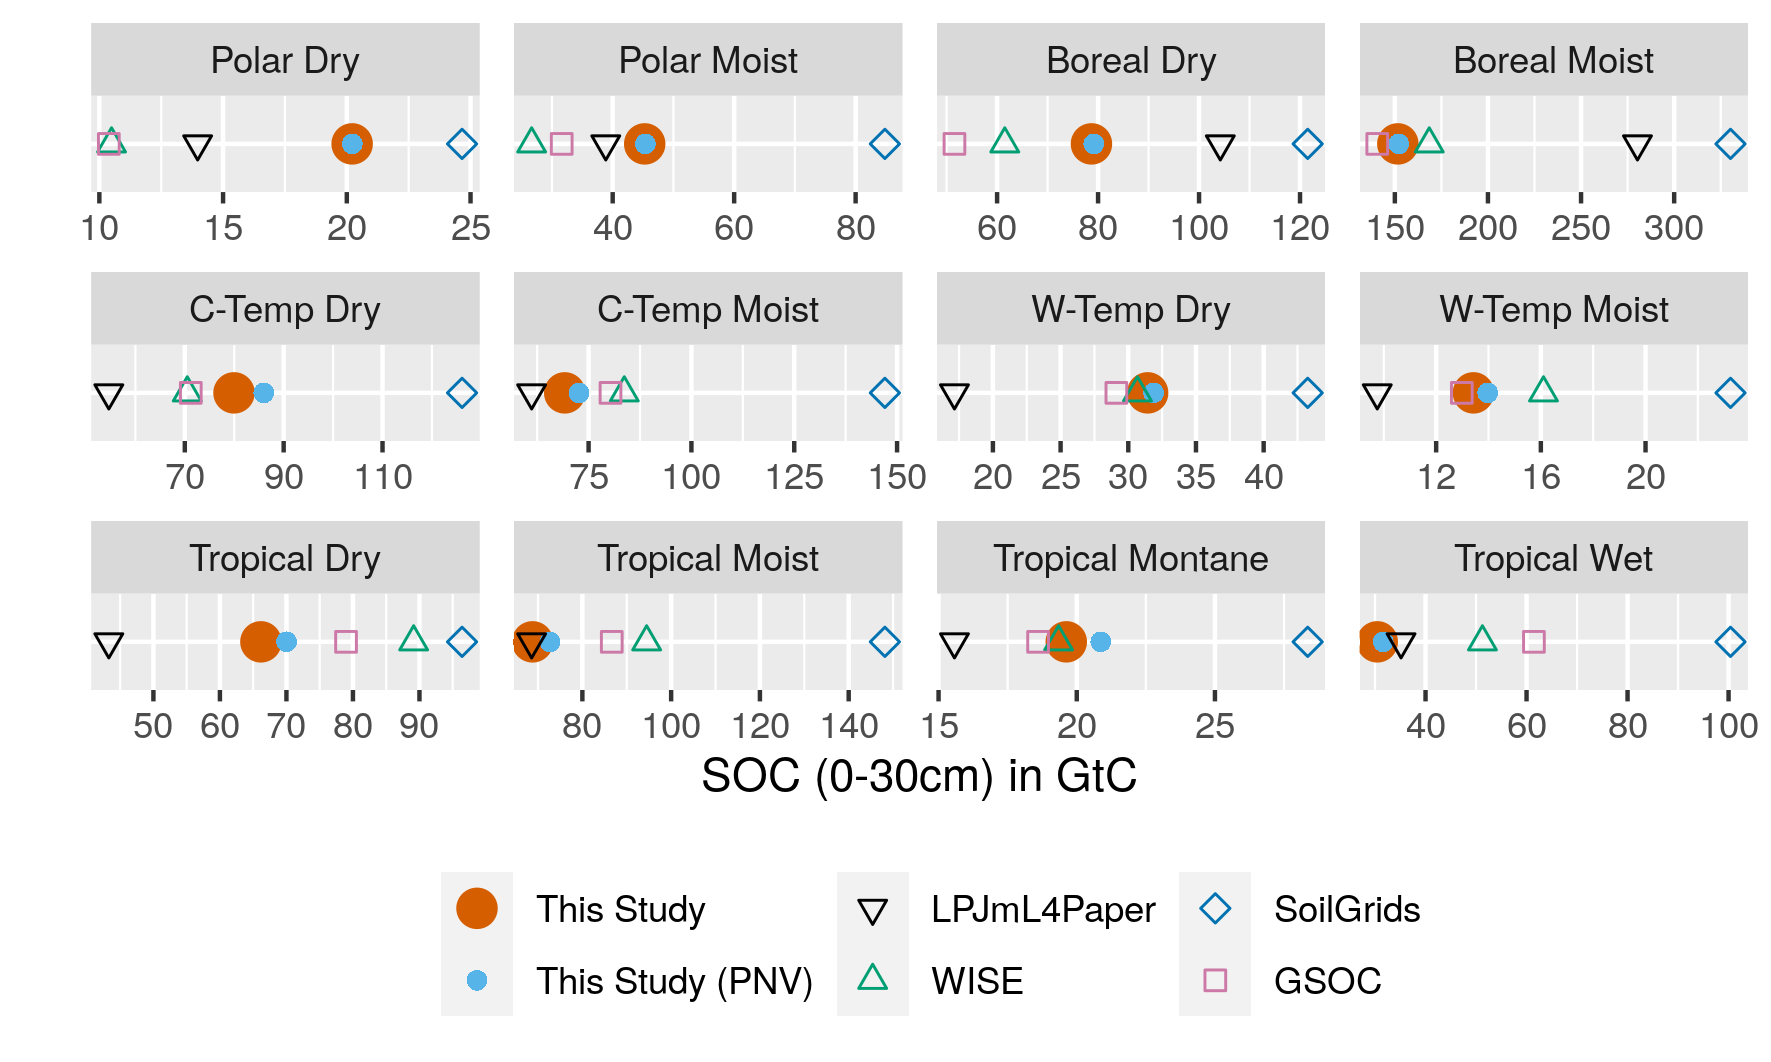
\includegraphics[width=16cm]{../ResultNotebooks/Output/Images/reg_comparisonfigure} 
\caption{Modelled as well as data based estimation for climate zone specific SOC stock in GtC for the first 30 cm of soil aggregated over all land area: SoilGrids, GSOC and WISE do not consider changes over time and rely on soil profile data gather over a long period of time, which makes it hard to pinpoint a specific year to these SOC estimations. In this context they will be compared to modelled data (LPJmL4, this study) for the year 2010. PNV denotes the potential natural vegetation state without considering human cropping activities, calculated as reference stock within our model. We use the climate zone specification of the IPCC \citep{eggleston_ipcc_2006}.}
\label{fig:SOCreg}
\end{figure}

\begin{figure}[H]
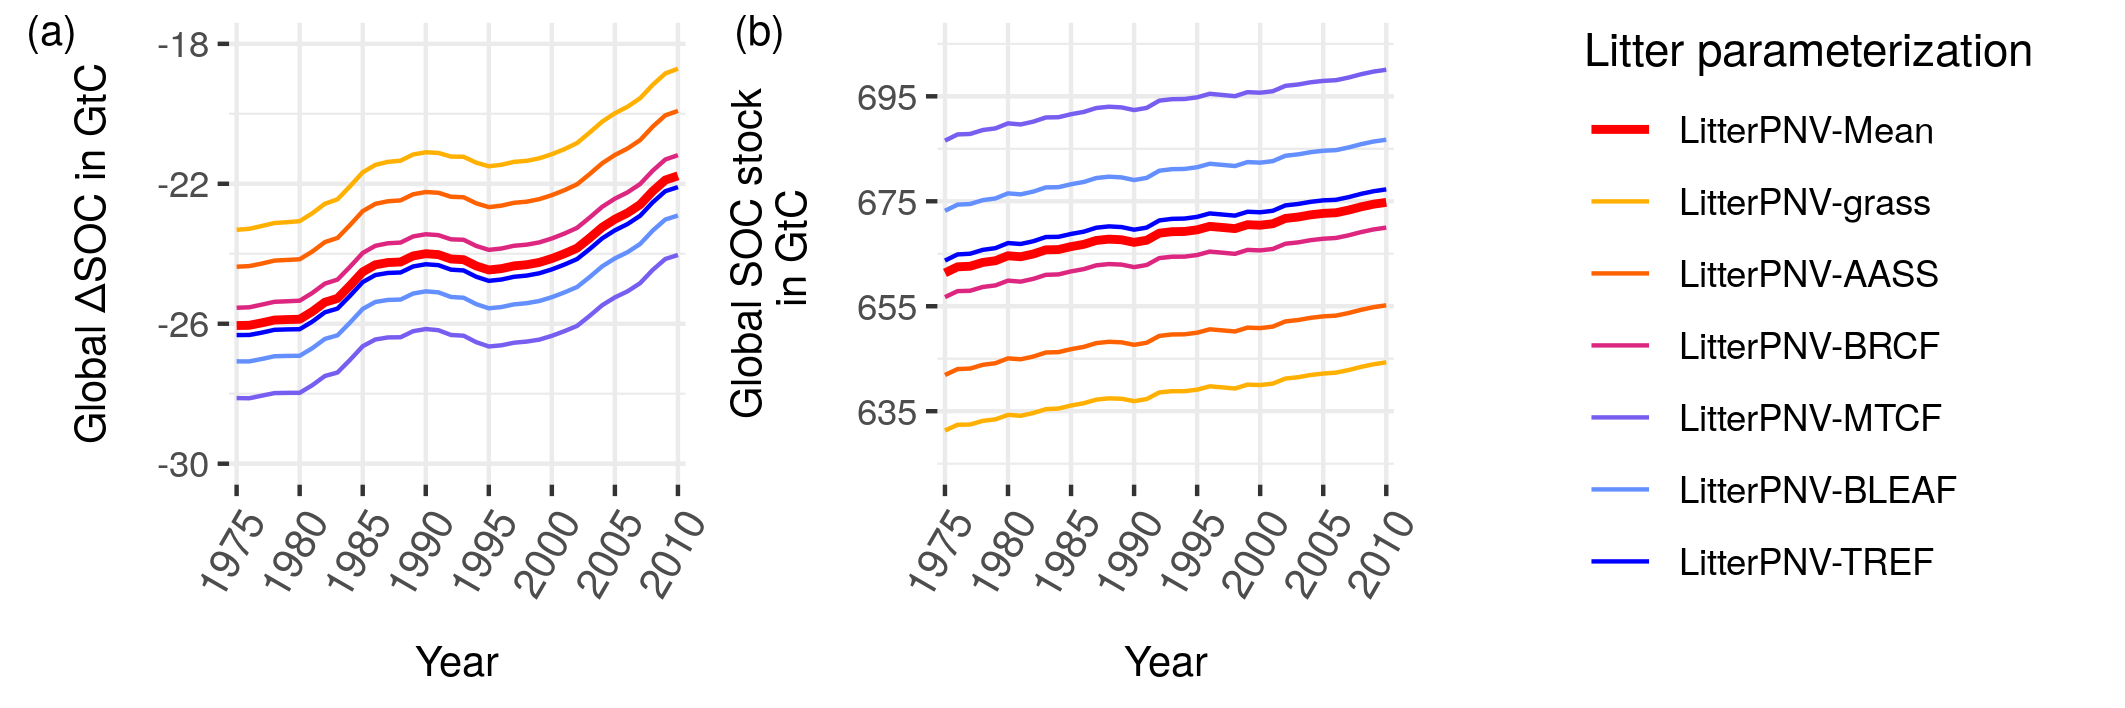
\includegraphics[width=16cm]{../ResultNotebooks/Output/Images/scenario_litter} 
\caption{Global $\Delta SOC$ for different litter parameterization choices: Whereas perennial grasses (scenario name \textit{LitterPNV-PerennialGrasses}) are given by the IPCC guidelines \citep{calvo_buendia_ipcc_2019}, we used CENTURY configuration file for woody biomass parameterization (see tree.100 in \citealt{century_model_2000}). \textit{LitterPNV-CenturyAverage} forms the baseline parameterization as used within the study and is calculated as the average over all tree compartments and tree types equally. Litter parameterization has the ability to change global SOC stocks and SOC debt, but is robust concerning trends and sequestration rates.}
\label{fig:SOClitter}
\end{figure}
\noappendix

%%%%%%%%%%%%%%%%%%%%%%%%%%%%%%%%%%%%%%%%%%
\authorcontribution{KK, BLB and AP designed the study and the model idea. KK wrote the code build on work of BLB, IW. JPD revised and improved the model code. CM, JH and SR provided the LPJmL simulation data. KK wrote the paper with important contributions of BLB and CM. MK, JS, SR and IW provided extensive feedback to outline of the study. All authors discussed the results and commented on the manuscript.} %% optional section

%%%%%%%%%%%%%%%%%%%%%%%%%%%%%%%%%%%%%%%%%%
\competinginterests{The authors declare no competing interests.} %% this section is mandatory even if you declare that no competing interests are present

%%%%%%%%%%%%%%%%%%%%%%%%%%%%%%%%%%%%%%%%%%

%%%%%%%%%%%%%%%%%%%%%%%%%%%%%%%%%%%%%%%%%%
\begin{acknowledgements}
Thanks to Vera Porwollik for contributing the time resolved tillage data set based on her previous work. Additional thanks to the rticles contributors for providing a R Markdown template. The authors thank for the data provided by FAOSTAT and LUH2v2. The work of KK was funded by the DFG Priority Program ``Climate Engineering: Risks, Challenges, Opportunities?'' (SPP 1689) and specifically the CEMICS2 project (grant no. ED78/3-2). The research leading to these results has received funding for BLB from the European Union's Horizon 2020 research and innovation program under grant agreement no. 776479 (COACCH) and no. 821010 (CASCADES). The work of SR, JS and IW was also supported by CLIMASTEPPE (01DJ8012), EXIMO (01LP1903D) and FOCUS (031B0787B) funded by the German Federal Ministry of Education and Research (BMBF). The input of PS, MK and MD contributes to the Soils-R-GGREAT project (NE/P019455/1) and CIRCASA (EU H2020; grant agreement no. 774378).
\end{acknowledgements}

%% REFERENCES
%% DN: pre-configured to BibTeX for rticles

%% The reference list is compiled as follows:
%%
%% \begin{thebibliography}{}
%%
%% \bibitem[AUTHOR(YEAR)]{LABEL1}
%% REFERENCE 1
%%
%% \bibitem[AUTHOR(YEAR)]{LABEL2}
%% REFERENCE 2
%%
%% \end{thebibliography}

%% Since the Copernicus LaTeX package includes the BibTeX style file copernicus.bst,
%% authors experienced with BibTeX only have to include the following two lines:
%%
\bibliographystyle{copernicus}
\bibliography{SOCbudget.bib}
%%
%% URLs and DOIs can be entered in your BibTeX file as:
%%
%% URL = {http://www.xyz.org/~jones/idx_g.htm}
%% DOI = {10.5194/xyz}


%% LITERATURE CITATIONS
%%
%% command                        & example result
%% \citet{jones90}|               & Jones et al. (1990)
%% \citep{jones90}|               & (Jones et al., 1990)
%% \citep{jones90,jones93}|       & (Jones et al., 1990, 1993)
%% \citep[p.~32]{jones90}|        & (Jones et al., 1990, p.~32)
%% \citep[e.g.,][]{jones90}|      & (e.g., Jones et al., 1990)
%% \citep[e.g.,][p.~32]{jones90}| & (e.g., Jones et al., 1990, p.~32)
%% \citeauthor{jones90}|          & Jones et al.
%% \citeyear{jones90}|            & 1990

\end{document}
